%=========================================================================
% Report for the Intelligent Distributed Systems course
% Universita' degli Studi di Trento - Prof. D. Fontanelli
%
% Compilation:  pdflatex main_eng -> pdflatex main_eng   (two passes, for the
%               cross-references). No bibtex: the bibliography is inline with
%               the thebibliography environment.
%=========================================================================
\documentclass[conference,9pt]{IEEEtran}

\usepackage[T1]{fontenc}
\usepackage[utf8]{inputenc}
\usepackage[english]{babel}
\usepackage{amsmath,amssymb}
\usepackage{graphicx}
\usepackage{booktabs}
\usepackage{algorithm}
\usepackage{algpseudocode}
\usepackage{balance}
\usepackage{xcolor}

% Margins reduced on all four sides with respect to the IEEEtran default, to
% keep the document within the 8-page limit.
\usepackage[a4paper,top=1.4cm,bottom=1.6cm,left=1.4cm,right=1.4cm,
            columnsep=0.55cm]{geometry}

% Internal references, citations and URLs in blue.
\definecolor{linkblue}{RGB}{0,64,168}
\usepackage[colorlinks=true,linkcolor=linkblue,citecolor=linkblue,
            urlcolor=linkblue,filecolor=linkblue,breaklinks=true]{hyperref}

% Compacted spacing around floats and equations: with 24 numbered equations and
% 12 floats, the default values waste almost a page.
\setlength{\textfloatsep}{6pt plus 2pt minus 2pt}
\setlength{\floatsep}{6pt plus 2pt minus 2pt}
\setlength{\intextsep}{6pt plus 2pt minus 2pt}
\setlength{\abovedisplayskip}{4pt plus 2pt minus 2pt}
\setlength{\belowdisplayskip}{4pt plus 2pt minus 2pt}
\setlength{\abovedisplayshortskip}{2pt}
\setlength{\belowdisplayshortskip}{2pt}

\floatname{algorithm}{Algorithm}
\renewcommand{\algorithmicrequire}{\textbf{Inputs:}}
\renewcommand{\algorithmicensure}{\textbf{Outputs:}}

\begin{document}

\title{Collaborative Localization and Formation Control\\
of a Fleet of Snow Groomers in GPS-Denied Environments}

\author{\IEEEauthorblockN{Alberto Dal Bosco [student no.\ 258028]}
\IEEEauthorblockA{Department of Industrial Engineering\\
University of Trento, Italy\\
alberto.dalbosco@studenti.unitn.it}
\thanks{Final report for the \emph{Intelligent Distributed Systems} course
[146033], Academic Year 2024/2025, Prof.\ D.\ Fontanelli.}}

\maketitle

\begin{abstract}
Ski slope grooming is carried out at night, on snow-covered ground and in areas
where satellite coverage is often degraded by narrow valleys, woods and ski
lifts. Under these conditions a fleet of snow groomers must keep a precise
formation without being able to rely on a continuous absolute reference and
without a central computer.
This work presents a decentralized architecture in which
every vehicle estimates its own pose with a local \emph{Extended Kalman Filter},
keeps the formation with a \emph{linear consensus} protocol on the
communication graph, and takes part in a distributed \emph{weighted least
squares} (D-WLS) estimation of a characteristic terrain parameter.
The architecture was developed incrementally and validated in a MATLAB
simulator that includes GPS-denied zones, Ultra-Wideband (UWB) anchors
positioned by GDOP minimization, an incomplete communication graph, sensors at
their real frequencies and a channel with variable latency and packet loss.
The results are obtained from a Monte Carlo campaign of 50 repetitions, and are
reported as mean and standard deviation.
The results show that in a blind zone the fleet reduces the trace of the
position covariance by a factor of 27 with respect to open-sky navigation with
a standard GNSS, and that cooperation improves by up to 8 times the
uncertainty on the terrain parameter of the least instrumented vehicles.
\end{abstract}

%=========================================================================
\section{Introduction}
%=========================================================================

Snowcats, or snow groomers, are large tracked vehicles (about 5\,m on the
tracks, 9\,m with tiller and blade) that work as a team to prepare ski slopes.
The work almost always takes place at night and on low-grip ground, and the
quality of the result depends on keeping a precise distance between the
vehicles.

\subsection{Problem formulation}

Consider a fleet of $N$ ground vehicles moving on a flat map of
$500 \times 500$\,m containing some zones where the GNSS signal cannot be
received because of narrow valleys, tree cover and artificial obstructions.
Each vehicle $i$ must:

\begin{enumerate}
\item continuously estimate its own pose and its own velocities, also declaring
      the uncertainty associated with the estimate;
\item keep an assigned position inside a rigid formation, using only
      information received from the neighbours reachable over the radio;
\item avoid collisions with the other members of the fleet;
\item contribute with the others to the identification of a characteristic
      terrain parameter, the same for everyone and constant in time.
\end{enumerate}

All of this without a central node, without any vehicle knowing the global
topology of the network, and in the presence of heterogeneous sensors working
at different frequencies.

\subsection{Organization of the document}

Sec.~\ref{sec:modelli} describes the vehicle model, the sensor model and the
communication network. Sec.~\ref{sec:soluzione} presents the proposed solution:
local estimator, formation control law and distributed estimator of the terrain
parameter. Sec.~\ref{sec:implementazione} reports the implementation details of
the simulator, including the generation of the environment.
Sec.~\ref{sec:risultati} collects the numerical results.
Sec.~\ref{sec:conclusioni} discusses strengths, limits and future developments.

%=========================================================================
\section{Adopted models}
\label{sec:modelli}
%=========================================================================

The system belongs to the category of \emph{distributed robotics} with
\emph{distributed perception}: the agents are mobile, each one carries its own
sensors, and the useful information arises from the combination of measurements
taken by different agents. The single vehicle is described first, then its
sensors, and finally the network that connects them.

\subsection{Vehicle model}

Each snow groomer is described by a kinematic model of \emph{unicycle} type
with a state vector extended to the velocities:

\begin{equation}
x_i = \begin{bmatrix} x_i & y_i & \theta_i & v_i & \omega_i \end{bmatrix}^T
\label{eq:stato}
\end{equation}

where $x_i, y_i$ are the Cartesian coordinates of the centre of mass [m],
$\theta_i$ the yaw angle with respect to the global $X$ axis [rad], $v_i$ the
longitudinal velocity [m/s] and $\omega_i$ the angular velocity [rad/s].

The inclusion of $v_i$ and $\omega_i$ \emph{in the state} rather than among the
inputs is not an arbitrary choice. On snow-covered ground the command sent to
the motors does not coincide with the actual velocity of the centre of mass
because of slip: using it as a deterministic input would introduce a
correlation between process noise and input, violating the assumptions of the
Kalman filter. By estimating the velocities the correct formulation is instead
preserved, and the ground is prepared for the slip model discussed in
Sec.~\ref{sec:conclusioni}.

The discrete-time motion model, with sampling step $T_s$, is:

\begin{equation}
x_{k+1} =
\begin{bmatrix}
x_k + v_k \cos(\theta_k)\,T_s\\
y_k + v_k \sin(\theta_k)\,T_s\\
\theta_k + \omega_k\,T_s\\
v_k\\
\omega_k
\end{bmatrix}
+ \varepsilon_k, \qquad \varepsilon_k \sim \mathcal{N}(0, Q_d)
\label{eq:moto}
\end{equation}

where the subscript $k$ denotes the instant $t_k = (k-1)T_s$, $\varepsilon_k$
is the process noise and $Q_d$ its covariance matrix (Sec.~\ref{sub:cwna}).
The last two rows constitute a \emph{random walk}: the model does not predict
how the velocities will change, and leaves it to the measurements to say so.

Actuation takes place through \emph{feedback linearization} on a point $P$
placed at a distance $b$ ahead of the centre of mass along the axis of the
vehicle. Given a desired Cartesian velocity $\dot{p}^{cmd} \in \mathbb{R}^2$
for that point, the physical commands are obtained as:

\begin{equation}
\begin{bmatrix} v^{cmd}\\ \omega^{cmd}\end{bmatrix}
=
\begin{bmatrix}
\cos\hat\theta & \sin\hat\theta\\[1ex]
-\dfrac{\sin\hat\theta}{b} & \dfrac{\cos\hat\theta}{b}
\end{bmatrix}
\dot{p}^{cmd}
\label{eq:fl}
\end{equation}

where $\hat\theta$ is the \emph{estimated} yaw and $b = 2.0$\,m, about half the
length of the vehicle. The transformation is invertible for every
$b \neq 0$ and allows the nonholonomic vehicle to be treated as a point that
can be freely commanded in the plane, which makes the theory of linear
consensus applicable without modifications.

\subsection{Sensor model}

Every vehicle is equipped with an AHRS (\emph{Attitude and Heading Reference
System}), with velocity sensors on the tracks, with a GNSS receiver, with a UWB
module for distance measurement and with a torque meter on the transmission
shaft. The measurement equations are the following.

\emph{AHRS}: it directly provides yaw and angular velocity,
\begin{equation}
z^{ahrs} = [\theta,\ \omega]^T + \delta^{ahrs}
\end{equation}

\emph{Track velocity}: the Hall effect sensor on the sprocket counts the
pulses and provides the angular velocity of the two tracks,
\begin{equation}
z^{enc} =
\begin{bmatrix}
\dfrac{v}{r} + \dfrac{L_c\,\omega}{2r}\\[2ex]
\dfrac{v}{r} - \dfrac{L_c\,\omega}{2r}
\end{bmatrix}
+ \delta^{enc}
\label{eq:enc}
\end{equation}
where $r = 0.5$\,m is the radius of the drive wheel and $L_c = 3.5$\,m the
track gauge, that is the distance between the two tracks. Eq.~\eqref{eq:enc}
assumes pure rolling, an assumption that will be removed in future
developments.

\emph{GNSS}: direct measurement of absolute position, available only outside
the blind zones,
\begin{equation}
z^{gnss} = [x,\ y]^T + \delta^{gnss}
\end{equation}

\emph{UWB ranging}: distance from a fixed anchor of known position
$p^{anc} = [X^{anc}, Y^{anc}]^T$, or from a neighbouring vehicle,
\begin{equation}
z^{uwb} = \sqrt{(x - X^{anc})^2 + (y - Y^{anc})^2} + \delta^{uwb}
\label{eq:uwb}
\end{equation}

\emph{Torque meter}: it measures the specific tractive effort, that is the
tractive force $F_{traz}$ normalized by the weight $W$ of the vehicle,
\begin{equation}
z^{traz} = \frac{F_{traz}}{W} = \mu_{terr} + c_{terr}\,v^2 + \delta^{traz}
\label{eq:traz}
\end{equation}
where $\mu_{terr}$ is the rolling resistance coefficient of the snowpack
[dimensionless] and $c_{terr}$ the term that grows with the square of the
velocity [s$^2$/m$^2$], related to snow compaction and to the resistance of the
tiller. They are the two parameters that the fleet must identify.

In all the equations $\delta$ denotes the measurement noise, Gaussian with zero
mean and with covariance $R$ reported in Table~\ref{tab:sensori}. The values
refer to components actually on the market in the off-highway sector, so that
the frequencies and the accuracies are not arbitrary numbers.

\begin{table}[t]
\centering
\caption{Adopted sensors, with real reference model, standard deviation and
native frequency. The simulation step is $1/T_s = 10$\,Hz.}
\label{tab:sensori}
\begin{tabular}{llrr}
\toprule
\textbf{Sensor} & \textbf{Model} & $\sigma$ & \textbf{Freq.}\\
\midrule
AHRS ($\theta$)      & Xsens MTi-3        & 0.05 rad     & 100 Hz\\
AHRS ($\omega$)      & Xsens MTi-3        & 0.02 rad/s   & 100 Hz\\
Track velocity       & Hall on sprocket   & 0.1 rad/s    & window\\
GNSS Master (RTK)    & u-blox ZED-F9P     & 0.2 m        & 5 Hz\\
GNSS Slave           & u-blox NEO-M8N     & 2.0 m        & 1 Hz\\
Ranging to anchor    & Qorvo DW1000       & 0.5 m        & $\sim$1 kHz\\
Ranging between veh. & Qorvo DW1000       & 0.6 m        & $\sim$1 kHz\\
Torque meter Master  & instrum.\ transm.  & 0.010        & 10 Hz\\
Torque meter Slave   & standard sensors   & 0.025        & 10 Hz\\
\bottomrule
\end{tabular}
\end{table}

Two asymmetries have to be motivated. The first is between Master and Slave:
only to the lead vehicle an RTK receiver and a torque meter of higher quality
are assigned. It is a design choice that makes observable how informative for
the network a vehicle with better equipment is during cooperation. The second
asymmetry is between ranging towards a fixed anchor ($\sigma_{uwb} = 0.5$\,m)
and ranging between vehicles ($\sigma_{collab} = 0.6$\,m): the antenna of the
vehicle is
lower and the effect of the metal platform is present on \emph{both} ends of
the link rather than on one only. The same physics also implies a
\emph{shorter range}, and it is the reason why the inter-vehicle radius
$r_{collab}$ is smaller than the one towards the anchors $r_{ancora}$.

\subsection{Communication network and graph}
\label{sub:grafo}

The network is modelled as an undirected graph
$\mathcal{G} = (\mathcal{N}, \mathcal{E})$, where $\mathcal{N}$ is the set of
the $N$ vehicles and $\mathcal{E}$ the set of the active radio links.
A link between two vehicles exists if their distance is smaller than the
communication radius $r_{collab} = 55$\,m. The procedure followed at every
simulation step is always the same:

\begin{enumerate}
\item the graph is built from the current positions, drawing an edge between
      every pair within $r_{collab}$;
\item from it the \textbf{adjacency matrix}
      $A \in \mathbb{R}^{N\times N}$ is extracted, with $a_{ij}=1$ if vehicles
      $i$ and $j$ see each other and $a_{ij}=0$ otherwise, together with the
      \textbf{degree matrix} $D = \mathrm{diag}(d_1,\dots,d_N)$, where
      $d_i = \sum_j a_{ij}$ is the number of neighbours of vehicle $i$;
\item the \textbf{Laplacian} $L = D - A$ and the \textbf{consensus matrix} $Q$
      are formed with the Metropolis-Hastings
      rule~\eqref{eq:metropolis};
\item the eigenvalues of the two matrices are computed, from
      $\det(L - \lambda I)=0$ and $\det(Q - \lambda I)=0$;
\item they are ordered with two different criteria: those of $L$ in
      \emph{increasing} order, so that $\lambda_1(L) = 0$ and $\lambda_2(L)$ is
      the algebraic connectivity; those of $Q$ by \emph{decreasing modulus}, so
      that $\lambda_1(Q) = 1$ and the essential spectral radius is
      $\rho_2 = |\lambda_2(Q)|$ by construction;
\item the two spectra are read \emph{separately}, according to
      Table~\ref{tab:spettri}.
\end{enumerate}

The Metropolis-Hastings rule \cite{xiao2004} assigns the weights as

\begin{equation}
q_{ij} =
\begin{cases}
\dfrac{1}{\max(d_i,d_j)+1} & \text{if } (i,j) \in \mathcal{E},\ i \neq j\\[1.5ex]
1 - \sum_{k \neq i} q_{ik} & \text{if } i = j\\[0.5ex]
0 & \text{otherwise}
\end{cases}
\label{eq:metropolis}
\end{equation}

where $q_{ij}$ is the weight that vehicle $i$ assigns to the information
received from $j$. Every node computes them knowing only its own degree and the
one of its direct neighbours: no knowledge of the global topology is required.
The resulting $Q$ is symmetric and therefore \emph{doubly stochastic} (rows and
columns sum to one), a necessary condition for the consensus to converge to the
exact arithmetic mean and not to an arbitrary weighted combination. The global
matrices $A$, $D$, $L$ and $Q$ exist only in the simulator, as an analysis
tool: on board the vehicle runs the component-wise form, summing the
contributions of only those nodes from which it has received a packet.

\begin{table}[t]
\centering
\caption{The two spectra and their meaning. They move in opposite directions: a
well connected network has $\lambda_2(L)$ large and $\rho_2$ small.}
\label{tab:spettri}
\begin{tabular}{lll}
\toprule
 & \textbf{Laplacian $L$} & \textbf{Metropolis $Q$}\\
\midrule
Use            & formation control    & distributed estimation\\
Time           & continuous           & discrete\\
Ordering of $\lambda_i$ & increasing  & decreasing modulus\\
Equilibrium cond. & $\lambda_1(L)=0$  & $\lambda_1(Q)=1$\\
\# connected comp. & $mol(\lambda_1(L))$   & $mol(\lambda_1(Q))$\\
Indicator      & $\lambda_2(L)$: connectivity & $\rho_2=|\lambda_2(Q)|$: speed\\
\bottomrule
\end{tabular}
\end{table}

The distinction matters because the two values answer different questions:
$\lambda_2(L)$ says \emph{how rigid} the formation is and fixes the time
constant of the control (Sec.~\ref{sub:consenso}), while $\rho_2$ says
\emph{how slow} the consensus is and fixes the number of radio exchanges needed
(Sec.~\ref{sub:dwls}).

%=========================================================================
\section{Proposed solution}
\label{sec:soluzione}
%=========================================================================

\subsection{Local pose estimation: EKF}

Every vehicle runs on board an \emph{Extended Kalman Filter} (EKF) in the
formulation of Thrun \emph{et al.} \cite{thrun2005}. The adopted notation is
the following: $\bar\mu_k$ and $\bar\Sigma_k$ are the \emph{a priori}
(predicted) estimate and covariance, $\mu_k$ and $\Sigma_k$ the \emph{a
posteriori} ones, $A_k = \partial f/\partial x$ and
$C_k = \partial h/\partial x$ the Jacobians of the motion and measurement
models, $K_k$ the Kalman gain.

The \textbf{prediction} step propagates~\eqref{eq:moto} and the covariance:
\begin{equation}
\bar\mu_k = f(\mu_{k-1}), \qquad
\bar\Sigma_k = A_k \Sigma_{k-1} A_k^T + Q_d
\end{equation}

The \textbf{correction} step fuses the measurement $z_k$:
\begin{align}
S_k &= C_k \bar\Sigma_k C_k^T + R_k\\
K_k &= \bar\Sigma_k C_k^T S_k^{-1}\\
\mu_k &= \bar\mu_k + K_k\,(z_k - h(\bar\mu_k))\\
\Sigma_k &= (I - K_k C_k)\,\bar\Sigma_k
\end{align}
where $S_k$ is the innovation covariance and $R_k$ that of the measurement
noise. Note the absence of the term $B_k u_k$ in the prediction: as argued
above, the velocities are states and not inputs.

The choice of the EKF over a UKF was checked on the criterion that matters,
that is how much the function curves within $\pm 3\sigma$: the linearization
error is $\tfrac{1}{2}v T_s \sigma_\theta^2 \approx 8\cdot10^{-6}$\,m per step,
three orders of magnitude below the process noise. The two solutions would be
indistinguishable, and the UKF would pay 11 propagations per step.

From the architectural point of view what matters is that the measurement
vector $z_k$ has \textbf{variable dimension}: at every step only the available
rows are appended, that is the GNSS if the receiver has produced a solution
outside the blind zones, one row for every UWB anchor in sight and one for
every neighbour in range. With the EKF it is enough to append rows to $z_k$,
$C_k$ and $R_k$; with the UKF the unscented transform would have to be run
again at every change of configuration.

\subsection{Process noise in CWNA form}
\label{sub:cwna}

The matrix $Q_d$ is not a constant diagonal but is rebuilt dynamically at every
step according to the CWNA (\emph{Continuous White Noise Acceleration}) model
\cite{barshalom2001}. The motivation is purely kinematic: in the unicycle model
the coordinates $x$ and $y$ do not possess an independent stochastic dynamics,
but evolve only through the propagation of the uncertainty on $v$ and $\theta$.
A diagonal $Q_d$ would inject noise directly on $x$ and $y$, that is it would
state that the vehicle moves sideways even when standing still.

In the CWNA model the noise enters on the \emph{accelerations}, where slip acts
physically, and propagates to the position through the model:
\begin{equation}
Q_d = \int_0^{T_s} e^{A\tau}\,\Gamma\,Q_c\,\Gamma^T e^{A^T\tau}\,d\tau
\label{eq:cwna}
\end{equation}
where $Q_c$ is the spectral density of the continuous-time noise and $\Gamma$
the matrix that distributes it over the states. Freezing $\theta$ over the
sampling interval, which is legitimate since with $T_s = 0.1$\,s and
$\omega \leq 0.6$\,rad/s the angle changes at most by 3.4$^\circ$, the integral
is solved in closed form.

The result is \emph{not} diagonal: it contains the position--velocity
correlations, physical information that a diagonal would discard. The three
noise channels are $q_a = 0.10$\,m$^2$/s$^3$ on the longitudinal acceleration,
$q_\alpha = 0.01$\,rad$^2$/s$^3$ on the angular one and
$q_{lat} = 0.02$\,m$^2$/s on the lateral drift. The last one is
indispensable: the unicycle is nonholonomic and without it $Q_d$ turns out
singular (rank 4 out of 5), with the uncertainty perpendicular to the direction
of travel never growing. The closed form is verified against the exact Van Loan
discretization, with a relative error of $4\cdot10^{-4}$.

\subsection{Formation control through consensus}
\label{sub:consenso}

The formation is defined by a set of desired positions
$p_i^{des} \in \mathbb{R}^2$ and by the corresponding offsets
$\Delta_{ij} = p_i^{des} - p_j^{des}$. The control law that governs the
Cartesian velocity $u_i \in \mathbb{R}^2$ commanded to vehicle $i$ is
structured as a consensus protocol:

\begin{equation}
u_i = -K_{cons} \sum_{j \in \mathcal{N}_i} a_{ij} \Big[(p_i - p_j) - \Delta_{ij}\Big]
\label{eq:consenso}
\end{equation}

where $K_{cons} > 0$ is the proportional gain [1/s], $\mathcal{N}_i$ is the set
of the neighbours in radio range and $a_{ij}$ is the element of the adjacency
matrix.

In this law the adjacency weights $a_{ij}$ are used and \emph{not} the
Metropolis weights $q_{ij}$. The law operates on \emph{differences}, therefore
the equilibrium of the formation is guaranteed for any set of weights
$a_{ij} \ge 0$ and there is no need either to normalize or to define a
self-weight $a_{ii}$. The weights $q_{ij}$ are instead born to build a
stochastic matrix, where the agent replaces its own information with an
average: using them in the control would mean discarding the self-weight
$q_{ii}$, destroying stochasticity, and tying the gain of the controller to the
local topology.

By introducing the translated variable $\tilde p_i = p_i - p_i^{des}$, the
error becomes $\tilde p_i - \tilde p_j$ and the equation is rewritten in
compact matrix form as:

\begin{equation}
u = -K_{cons}\,(L \otimes I_2)\,\tilde p
\label{eq:consenso_matriciale}
\end{equation}

that is \emph{exactly} the linear consensus protocol of the course
\cite{fontanelli_notes}, where $\otimes$ is the Kronecker product and $I_2$ the
$2\times 2$ identity matrix. Keeping the formation reduces to a consensus
problem on translated coordinates, whose error decays exponentially with a time
constant:

\begin{equation}
\tau = \frac{1}{K_{cons}\,\lambda_2(L)}
\label{eq:tau}
\end{equation}

where $\lambda_2(L)$ is the algebraic connectivity, that is the second smallest
eigenvalue of the Laplacian. This relation was used as a design constraint in
order to guarantee uniform responsiveness. Moving from the three-vehicle
formation with complete graph ($\lambda_2(L) = 3.000$) to the five-vehicle one
with sparse graph ($\lambda_2(L) = 0.697$), with the same gain the settling
time $\tau$ would rise from 2.22\,s to 9.56\,s. The gain $K_{cons}$ was
therefore recomputed topology by topology in order to keep $\tau$ unchanged,
obtaining for the final graph the value $K_{cons} = 0.646$.

To the continuous-time stability two constraints are added for the
discrete-time implementation. The first concerns Euler integration: the state
transition matrix becomes $\Phi = I - K_{cons} T_s L$, whose eigenvalues are
$\lambda_{i}(\Phi) = 1 - K_{cons} T_s \lambda_{i}(L)$. To guarantee asymptotic
stability it must hold that $-1 < \lambda_{i}(\Phi) < 1$ for every $i$, a
condition that reduces to $K_{cons} T_s \lambda_{max}(L) < 2$, where
$\lambda_{max}(L)$ is the largest eigenvalue of the Laplacian. With the
parameters of the project that product is 0.278, well within the limit. The
second constraint concerns the theoretical limit of tolerance to the
communication delay $\tau_d$ \cite{olfati2004}:

\begin{equation}
\tau_d < \frac{\pi}{2\,K_{cons}\,\lambda_{max}(L)}
\label{eq:ritardo}
\end{equation}

For the adopted topology, the maximum delay tolerable before the system loses
stability and starts to oscillate is 565\,ms, that is slightly more than five
sampling steps.

\subsection{Collision avoidance}

A repulsive term based on artificial potential fields \cite{khatib1986} is
superimposed on the consensus. Consensus and repulsion are not two distinct
controllers but the two terms of a single potential $U = U_{cons} + U_{rep}$,
of which the control law is the antigradient: the consensus is the attractive
potential, whose minimum coincides with the desired formation, and the FIRAS
function provides the repulsive one. Denoting by $d_{ij}$ the distance between
two vehicles and by $d_{safe}$ the safety threshold:

\begin{equation}
u_i^{rep} = \sum_{j \neq i} k_{rep}
\left(\frac{1}{d_{ij}} - \frac{1}{d_{safe}}\right)\frac{1}{d_{ij}^2}\,
\frac{p_i - p_j}{d_{ij}}
\qquad \text{if } d_{ij} < d_{safe}
\label{eq:firas}
\end{equation}

where $k_{rep}$ is the repulsive gain, obtained by inverting a design
requirement which prescribes that at half the safety distance the repulsion be
worth 3\,m/s.

Two constraints must hold, both imposed by an \texttt{assert} at
initialization. The first, $d_{safe} < \min_{i \neq j}\lVert\Delta_{ij}\rVert$,
prevents the repulsion from staying active in the desired configuration, which
would make the formation unreachable. The second, $d_{safe} < r_{collab}$,
guarantees that the neighbour is in range when it needs to be pushed away: the
repulsion requires the \emph{direction}, which only comes from the radio
packet.

\subsection{Distributed estimation of the terrain parameter (D-WLS)}
\label{sub:dwls}

Alongside the pose estimation, which is dynamic and local to each vehicle, the
fleet solves a second problem of a different nature: identifying the pair
$x_{terr} = [\mu_{terr},\ c_{terr}]^T$ of~\eqref{eq:traz}, the same for
everyone and constant in time. Since it is a constant and non-stochastic
parameter, the solution applied is that of \emph{distributed weighted least
squares} (D-WLS) \cite{fontanelli_notes}, since a distributed Kalman filter
would be needed only if the quantity had a dynamics of its own.

Since the noises of the different vehicles are uncorrelated, the global matrix
$R$ is block diagonal and the centralized WLS solution decomposes into sums of
purely local contributions. Every vehicle builds its own
\textbf{information pair}:

\begin{equation}
F_i = C_i^T R_i^{-1} C_i, \qquad a_i = C_i^T R_i^{-1} z_i
\label{eq:coppia}
\end{equation}

where $F_i \in \mathbb{R}^{2\times2}$ is the local \emph{information matrix},
$a_i \in \mathbb{R}^2$ the local \emph{information state},
$C_i = [1\ \ v_i^2]$ the regression row and $R_i$ the variance of the torque
meter. The contributions accumulate in time, which is equivalent to stacking
the rows of $C$ and the samples of $z$.

The two quantities are then averaged over the network through $q$ consensus
cycles with the weights~\eqref{eq:metropolis}, and the estimate is
reconstructed locally:

\begin{equation}
\hat x_{terr,i} = \big(F_i(q)\big)^{-1} a_i(q)
\label{eq:ricostruzione}
\end{equation}

\begin{algorithm}[t]
\caption{D-WLS run by vehicle $i$ at every step}
\label{alg:dwls}
\begin{algorithmic}[1]
\Require measurement $z^{traz}_i$, estimated velocity $\hat v_i$, degrees of the neighbours
\Ensure local estimate $\hat x_{terr,i}$ and its uncertainty
\State $C_i \gets [\,1 \quad \hat v_i^2\,]$
\State $F_i \gets F_i + C_i^T R_i^{-1} C_i$
      \Comment{local accumulation}
\State $a_i \gets a_i + C_i^T R_i^{-1} z^{traz}_i$
\State $F_i^{(0)} \gets F_i$; \quad $a_i^{(0)} \gets a_i$
      \Comment{copies are used}
\For{$t = 1$ \textbf{to} $q$}
  \State exchange $F_i^{(t-1)}, a_i^{(t-1)}$ with the neighbours
  \State $F_i^{(t)} \gets \sum_j q_{ij} F_j^{(t-1)}$
  \State $a_i^{(t)} \gets \sum_j q_{ij} a_j^{(t-1)}$
\EndFor
\State $\hat x_{terr,i} \gets \big(F_i^{(q)}\big)^{-1} a_i^{(q)}$
\State $\Sigma_{terr} \gets \big(N\,F_i^{(q)}\big)^{-1}$
      \Comment{here $N$ does \emph{not} cancel out}
\end{algorithmic}
\end{algorithm}

Three observations, summarized in Alg.~\ref{alg:dwls}.

\textbf{No vehicle can solve the problem alone.} The parameters are two and
every vehicle produces one scalar measurement per step, so its instantaneous
$F_i$ is an outer product of \emph{rank 1 out of 2}: the local problem is
singular. It becomes solvable only by joining measurements taken at different
velocities, provided by the formation (on a curved path the wings of the V
travel arcs of a different radius than the Master) and by the accumulation
along the mission.

\textbf{The factor $1/N$ cancels out in the estimate but not in the
covariance.} At convergence $F_i(q) = \frac{1}{N}\sum_l F_l$, and in the ratio
of~\eqref{eq:ricostruzione} the normalization disappears: the D-WLS \emph{does
not require knowing the cardinality of the network}. To declare the uncertainty
$\Sigma_{terr} = (N F_i(q))^{-1}$ is however needed, where the factor remains.

\textbf{The number of cycles $q$ is not a constant written by hand.} It is
dimensioned from the essential spectral radius:
\begin{equation}
q \geq \max\left(\left\lceil \frac{\log \epsilon}{\log \rho_2} \right\rceil,\
\mathrm{diam}(\mathcal{G})\right)
\label{eq:qcicli}
\end{equation}
where $\epsilon$ is the required tolerance on the residual disagreement between
the nodes and $\mathrm{diam}(\mathcal{G})$ the diameter of the graph, that is
the maximum number of hops between two nodes. The value $\epsilon = 10^{-4}$ is
adopted: the consensus residual has to be compared with the uncertainty of the
estimate, and with a relative standard deviation on $c_{terr}$ of the order of
10\% a disagreement of $10^{-4}$ is already three orders of magnitude below
what matters. With $\rho_2 = 0.826$, Eq.~\eqref{eq:qcicli} gives
$\lceil \log(10^{-4})/\log(0.826)\rceil = \lceil 48.1 \rceil = 49$ cycles.
The constraint on the diameter is necessary anyway: below that threshold the
information has not materially crossed the network. The result is then
truncated to the available radio budget, and an indicator signals when the
channel is no longer enough instead of silently producing a wrong number.

%=========================================================================
\section{Implementation details}
\label{sec:implementazione}
%=========================================================================

\subsection{Incremental development}

The work was organized by dividing it into successive phases, each of which
removes a single simplifying assumption and is validated before moving to the
next one. The choice made it possible to attribute every variation of the
results to a precise cause, instead of having to diagnose a complete system
that does not work as expected. Phase 1 develops the single vehicle with its
EKF; Phase 2 introduces the three-vehicle fleet, the consensus and the
collision avoidance; Phase 3 adds the GPS-denied zones, the UWB anchors and the
D-WLS; Phase 4, the arrival point of this work and the subject of the results,
removes the ideality of the network by introducing a sparse graph, sensors at
real frequency and a non-ideal channel.

Every phase is implemented in a self-contained MATLAB script, which shares with
the others a set of common functions (graph construction, Metropolis weights,
CWNA noise, D-WLS consensus).

\textbf{Monte Carlo campaign.} All the results of the following section are
obtained by repeating \textbf{50 times} the same configuration, changing only
the seed of the random number generator, fixed to the number of the repetition
so that the campaign is reproducible. The campaign does not duplicate the
simulation code: it runs the same Phase 4 script in batch mode, without
generating figures, and collects its variables at the end of every repetition.
The reason for repeating is concrete: a single run does not allow a property of
the system to be distinguished from a fluctuation of the noise, and for the
terrain estimation the difference turns out to be substantial.

\subsection{Environment generation and anchor placement}
\label{sub:ambiente}

The environment is not drawn by hand but generated by a dedicated script, with
a fixed random seed to make it reproducible. The nominal path is a sinusoid of
amplitude 100\,m that crosses the map along $Y$; the $n_{area} = 8$ GPS-denied
zones have their centre drawn uniformly on the map and their radius drawn in
$[45, 85]$\,m, so that the shadow areas are not all of the same size. The
\emph{critical points} are then selected, that is the points of the path that
fall inside at least one blind zone: they are the ones where the vehicle will
have to rely on UWB alone, and they are the only place where it makes sense to
optimize the position of the anchors.

The placement of the $n_{ancore} = 5$ anchors minimizes the average
\textbf{GDOP} (\emph{Geometric Dilution of Precision}) over the critical
points. Denoting by $C_{geom}$ the matrix that collects, for every anchor $m$
visible from point $p$, the unit vector of the line of sight:

\begin{equation}
C_{geom}^{(m)} = \frac{\big(p - p^{anc}_m\big)^T}{d_m},
\qquad
\mathrm{GDOP} = \sqrt{\mathrm{tr}\big[(C_{geom}^T C_{geom})^{-1}\big]}
\label{eq:gdop}
\end{equation}

where $C_{geom}^{(m)}$ is the row of $C_{geom}$ relative to anchor $m$ and
$d_m = \lVert p - p^{anc}_m\rVert$ is the distance from that anchor. The
GDOP is a dimensionless multiplicative factor: the resulting position
uncertainty is about $\mathrm{GDOP}\cdot\sigma_{uwb}$. With $n$ anchors visible
and well distributed in angle one has $C_{geom}^T C_{geom} = (n/2)\,I_2$ and
therefore $\mathrm{GDOP} = 2/\sqrt{n}$: it is 1.41 with two anchors, 1.00 with
four and 0.89 with five. A value around unity therefore indicates a healthy
geometry, while $\mathrm{GDOP} \to \infty$ signals that $C_{geom}^T C_{geom}$
is becoming singular and that one direction of the plane is no longer
observable.

\textbf{How many anchors are needed.} The answer is read in the rank of
$C_{geom}$, which has as many rows as the anchors in sight and two columns:

\begin{itemize}
\item \emph{a single anchor}: $C_{geom}^T C_{geom}$ has rank 1 and is
      singular, the GDOP diverges. The measurement constrains only the distance
      from the anchor, and the position remains free to slide along a circle;
\item \emph{two anchors}: the rank is full provided the two directions are not
      aligned, but geometrically the two circles intersect in \emph{two}
      points. The ambiguity remains, and is resolved by the fact that the EKF
      linearizes around the prediction and therefore chooses the branch
      consistent with the current estimate. It is the minimum with which the
      filter manages to work, and it is the threshold imposed as a penalty in
      the optimization;
\item \emph{three or more anchors}: the solution is unique even without relying
      on the prediction, and the GDOP goes down towards unity.
\end{itemize}

In the optimized configuration the vehicle in a blind zone always sees at least
three anchors, typically four or five, as shown by the upper panel of
Fig.~\ref{fig:covarianza}. The matrix $C_{geom} $ of~\eqref{eq:gdop}
\emph{coincides} moreover with the ranging rows of the Jacobian $C_k$ of the
EKF: the GDOP is a measure of the conditioning of the very same estimation
problem that the filter will have to solve at that point.

The optimization is entrusted to Nelder-Mead (through the \texttt{fminsearch}
function), with the installability constraint inside the map imposed as an
additive penalty. With five anchors the search space has ten dimensions, at the
limit of reliability of the method: the result is a local minimum, not the
global optimum.

\subsection{Simulation cycle and time convention}

In a closed-loop simulator estimation and control chase each other, and it is
necessary to fix without ambiguity to which instant every quantity refers. The
convention adopted is that $\hat x_k$ is the a posteriori estimate at $t_k$,
$z_k$ the measurement acquired at $t_k$ and $u_k$ the command applied in the
interval $[t_k, t_{k+1})$. Every iteration runs five blocks in this order:

\begin{enumerate}
\item \textbf{Broadcast}: every agent publishes its own state estimate on the
      network;
\item \textbf{Control}: $u_k$ computed from $\hat x_k$ alone;
\item \textbf{Plant}: advancement of the \emph{ground truth} for all;
\item \textbf{Sensors}: generation of $z_{k+1}$ from the ground truth at
      $t_{k+1}$;
\item \textbf{Estimation}: prediction and correction, obtaining $\hat x_{k+1}$.
\end{enumerate}

Two constraints justify this order. The \emph{causality of the control}: the
command that acts during $[t_k, t_{k+1})$ can depend only on $\hat x_k$. And
the \emph{temporal coherence of the innovation}: correcting a prediction
referred to $t_{k+1}$ with a measurement acquired at $t_k$ would introduce a
\emph{systematic} error of the order of $|v|T_s$, which is not represented in
$\Sigma$ and would invalidate the consistency analysis. Blocks 3 and 4 are two
distinct passes because the inter-vehicle distance measurements depend on the
real position of the neighbours.

\subsection{Channel model}

The pose packet exchanged at 10\,Hz arrives neither immediately nor always. The
delay is modelled as a Gaussian $\mathcal{N}(100\,\mathrm{ms},
(33\,\mathrm{ms})^2)$ truncated to $[0, 200]$\,ms, and the packet loss as a
Bernoulli event at 0.5\%. The symmetric Gaussian is not faithful to real
latencies, which are right-skewed, but it is \emph{conservative}: for the same
maximum it has a higher mean and stresses the system more.

Delay and loss combine into a single quantity, the \textbf{age} $\eta_{ij}$ of
the data that vehicle $i$ holds of $j$, expressed in steps. The simulator keeps
a single index $k_{rx}(i,j)$, that of the freshest packet received:

\begin{equation}
k_{rx}(i,j) \gets \max\Big(k_{rx}(i,j),\ \max\big(1,\ k - \lceil d/T_s \rceil\big)\Big)
\label{eq:krx}
\end{equation}

where $d$ is the delay drawn for that packet. The outer $\max$ prevents a late
packet from replacing a more recent datum already received; on a lost packet
the index does not advance and the datum ages on its own.

In the project two possible reactions to the delay are adopted:
\begin{enumerate}
\item \textbf{passive} handling: the old packet is used without applying
      corrections. It is the mode chosen for the formation consensus, where the
      delay is accepted because it stays well below the stability limit
      of~\eqref{eq:ritardo};
\item \textbf{active} handling: the position of the neighbour is propagated
      forward with its motion model, for the whole age of the packet. It is the
      mode chosen for the UWB mobile anchors, where comparing a distance
      measurement acquired now with a position referred to the past would
      introduce a systematic error equal to $|v_j|\,\eta_{ij} T_s$.
\end{enumerate}

No \emph{timestamping} with retroactive re-insertion into the filter buffer is
instead needed, because no vehicle transmits measurements of others: the delay
concerns the pose used as a reference, not a measurement of its own state
arrived out of sequence.

%=========================================================================
\section{Results}
\label{sec:risultati}
%=========================================================================

All the results refer to the final configuration (Phase 4):
$N = 5$ vehicles in a ``V'' formation 60\,m deep, communication radius
$r_{collab} = 55$\,m, anchor visibility radius $r_{ancora} = 150$\,m,
$n_{ancore} = 5$ fixed anchors, sensors at the frequencies of
Table~\ref{tab:sensori}, channel with delay and losses. The mission lasts
$1218.0 \pm 0.2$\,s (about 12\,180 samples at 10\,Hz) and takes place on the
map of Fig.~\ref{fig:mappa}. Where not indicated otherwise, the values are mean
and standard deviation over the 50 repetitions of the campaign.

\begin{figure}[t]
\centering
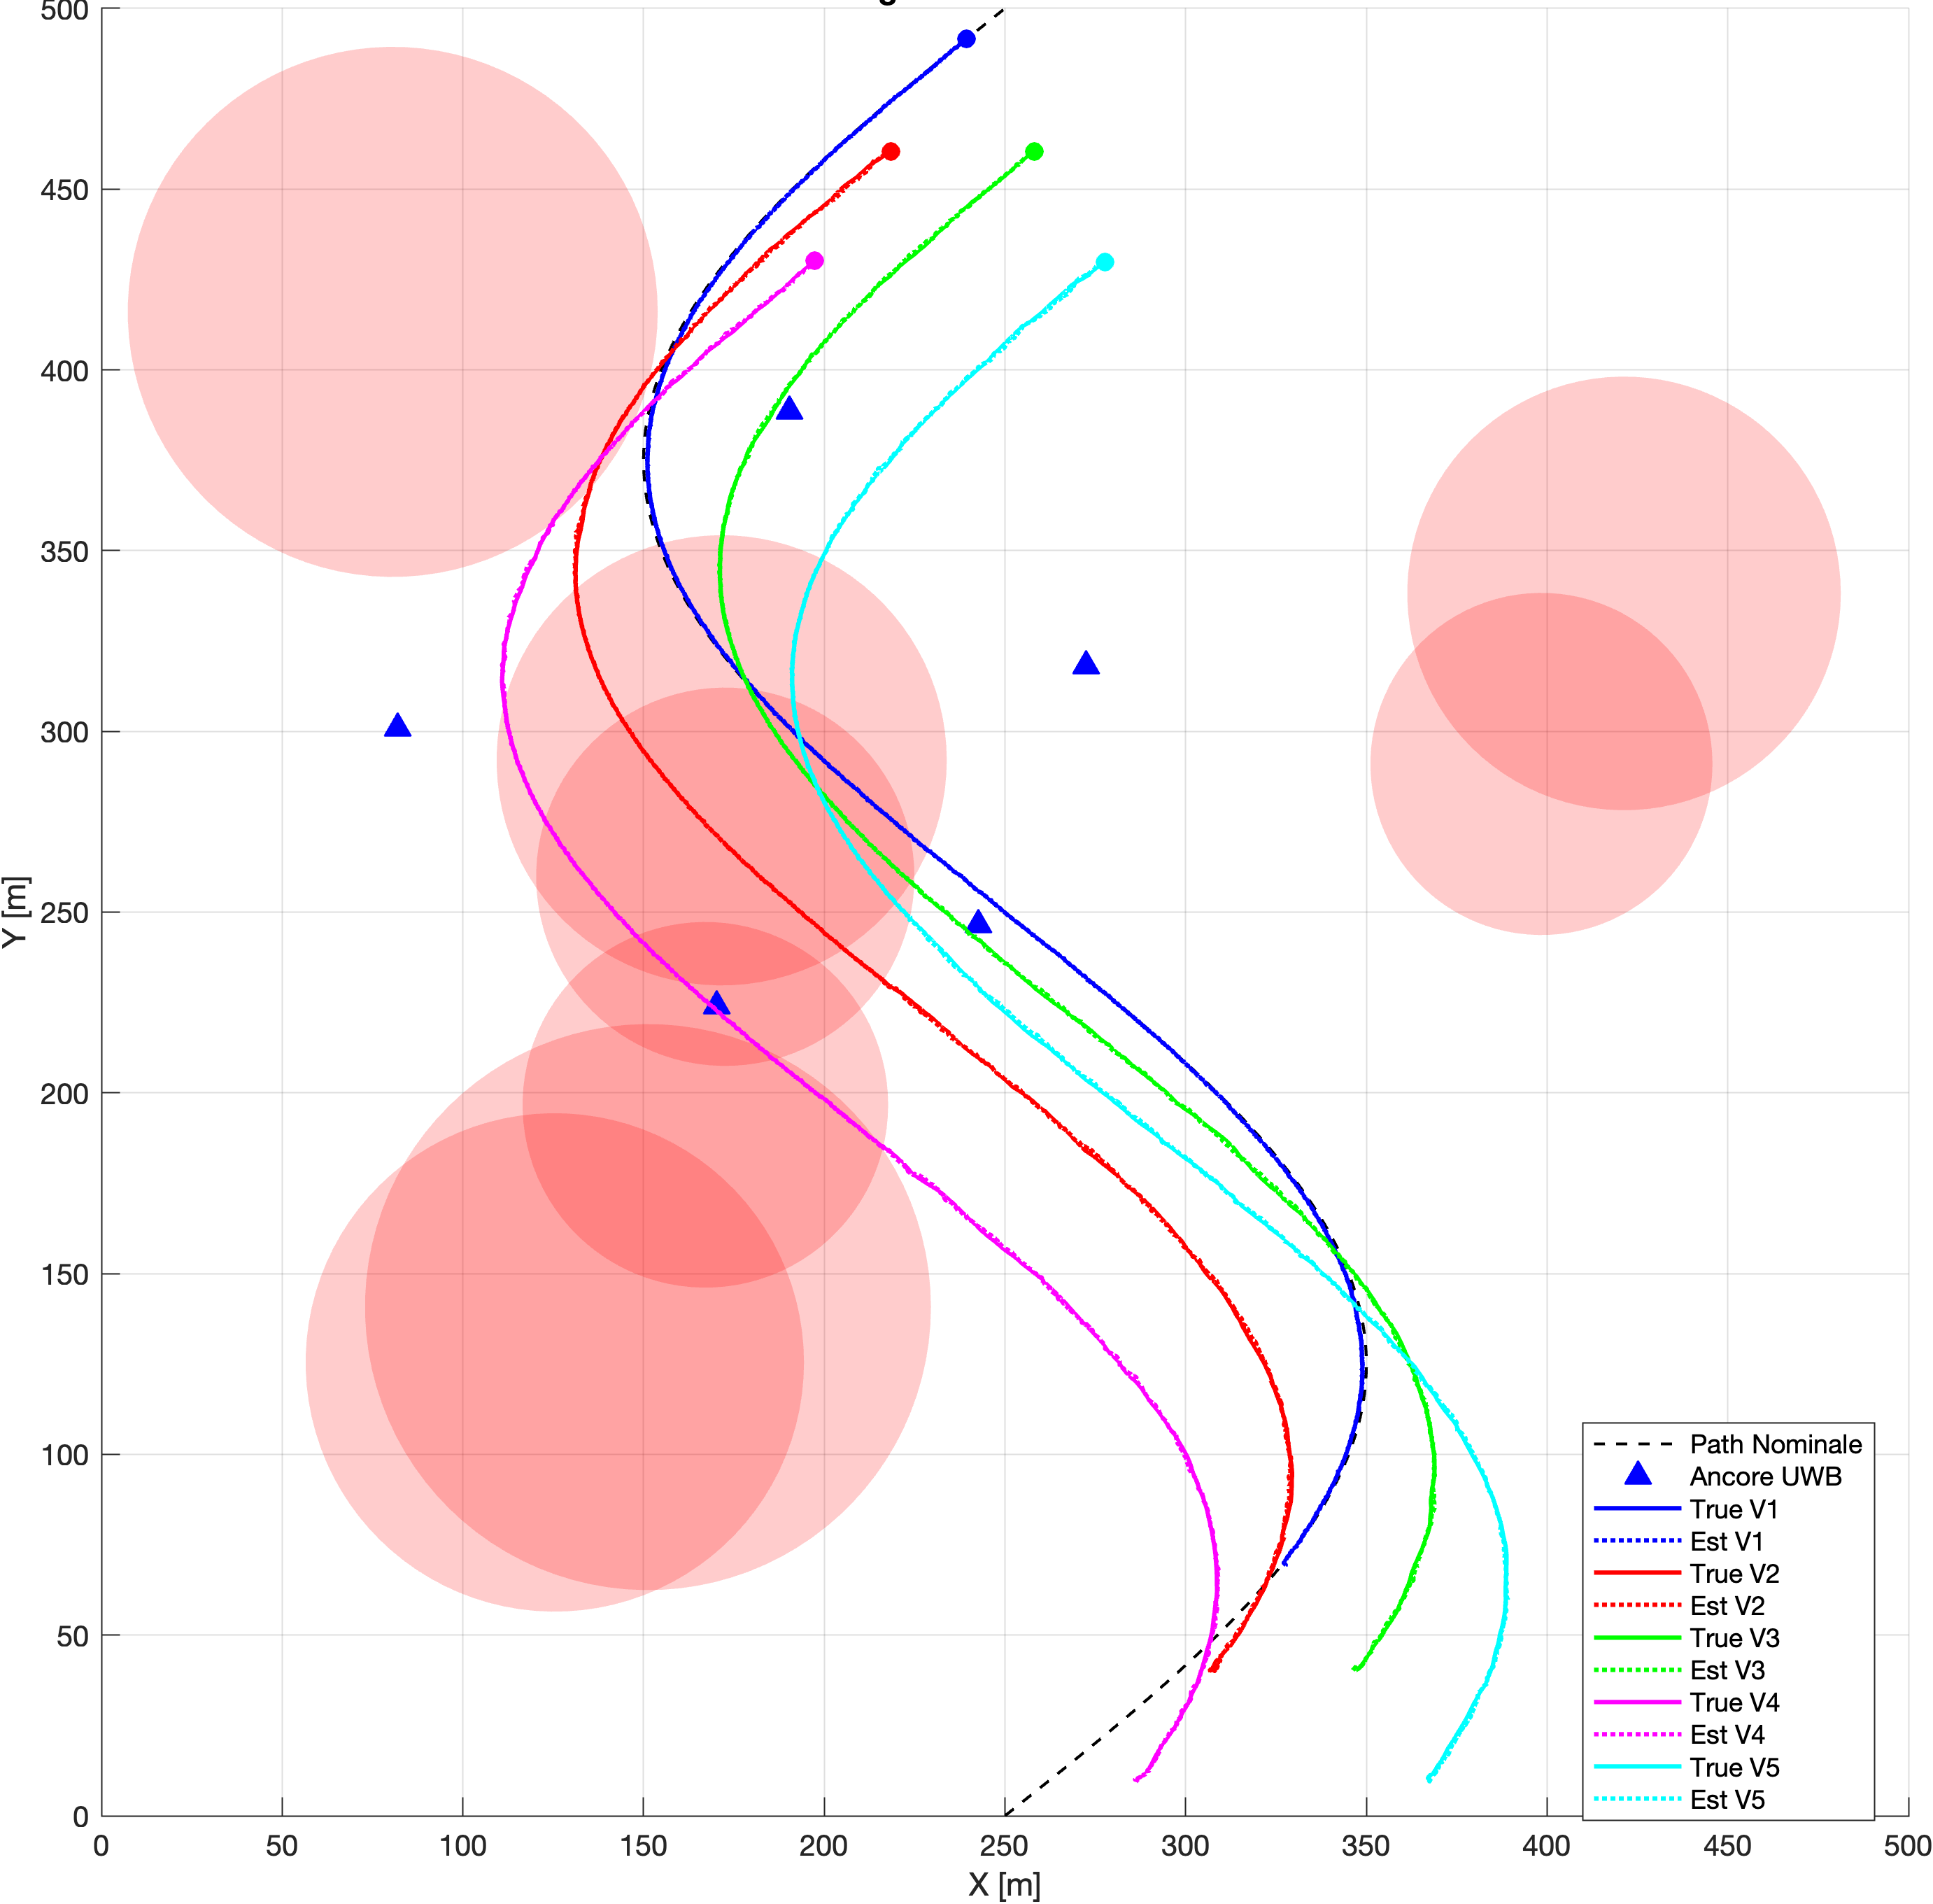
\includegraphics[width=0.95\columnwidth]{figure/1_mappa_navigazione.png}
\caption{Simulation scenario. Black dashed line: nominal path, followed by the
Master alone. Red circles: GPS-denied zones. Blue triangles: UWB anchors,
placed by GDOP minimization. Solid lines: real position of the five vehicles;
dotted lines: EKF estimate. The overlap between the two measures the quality of
the localization.}
\label{fig:mappa}
\end{figure}

\subsection{The communication graph becomes a constraint}

With $r_{collab} = 55$\,m and the five-vehicle formation, five pairs out of ten
do not see each other. The resulting topology is a chain
\texttt{V4--V2--V1--V3--V5} plus the edge \texttt{V2--V3}: V2 and V3 are
articulation points, and the failure of either one would detach an entire
branch. The spectral quantities, obtained with the procedure of
Sec.~\ref{sub:grafo}, are collected in Table~\ref{tab:grafo}.

\begin{table}[t]
\centering
\caption{Spectral properties of the graph, comparison between the
three-vehicle configuration with complete graph and the final five-vehicle
one.}
\label{tab:grafo}
\begin{tabular}{lrr}
\toprule
\textbf{Quantity} & \textbf{$N=3$, $K_3$} & \textbf{$N=5$, sparse}\\
\midrule
Active edges                       & 3 of 3 & \textbf{5 of 10}\\
Connectivity $\lambda_2(L)$        & 3.000  & \textbf{0.697}\\
Spectral radius $\rho_2=|\lambda_2(Q)|$ & 0.000 & \textbf{0.826}\\
Minimum eigenvalue $\lambda_{min}(Q)$ & 0.000 & $-0.076$\\
Connected components               & 1      & 1\\
Diameter                           & 1 hop & \textbf{3 hops}\\
Gain $K_{cons}$                    & 0.150  & \textbf{0.646}\\
Time constant $\tau$               & 2.22 s & 2.22 s\\
Discretization margin              & 0.045  & 0.278 (limit 2)\\
Consensus cycles $q$               & 1      & \textbf{49 of 50}\\
\bottomrule
\end{tabular}
\end{table}

The complete spectrum of $Q$ in the final configuration is
$[+1.000,\ +0.826,\ +0.654,\ +0.096,\ -0.076]$. The reading follows
Table~\ref{tab:spettri}: $\lambda_1(Q) = 1$ with unit multiplicity confirms that
the network is connected; $\rho_2 = 0.826$ measures the slowness of the
consensus; $\lambda_{min}(Q) = -0.076$, far from $-1$, rules out oscillatory
behaviours. On the Laplacian, $\lambda_1(L) = 0$ with multiplicity 1 gives the
same information on connectivity, while $\lambda_2(L) = 0.697$ quantifies the
rigidity of the formation.

The most significant jump is on the last row of the table. On a complete graph
the Metropolis rule gives $q_{ij} = 1/N$ for every pair, therefore
$\rho_2 = 0$ and the consensus converges in a single step: the distributed
estimation algorithms turn out exact with a single iteration. With the sparse
graph the dimensioning~\eqref{eq:qcicli} requires \textbf{49 cycles out of the
50 available}, that is 98\% of the allocated bandwidth. The consensus goes from
being a marginal item to being a design constraint, and the choice of the radio
radius becomes a trade-off between quality of the link and cost of the
communication.

The topology stays deterministic for the whole mission, as Fig.~\ref{fig:grafo}
shows: the nominal distances separate into two sharp groups,
36--41\,m and 66--81\,m, with a gap of 25\,m in between: the margin is
$+34\%$ on the active links and $-16\%$ on the absent ones, therefore the
formation error does not make them flicker.

\begin{figure*}[t]
\centering
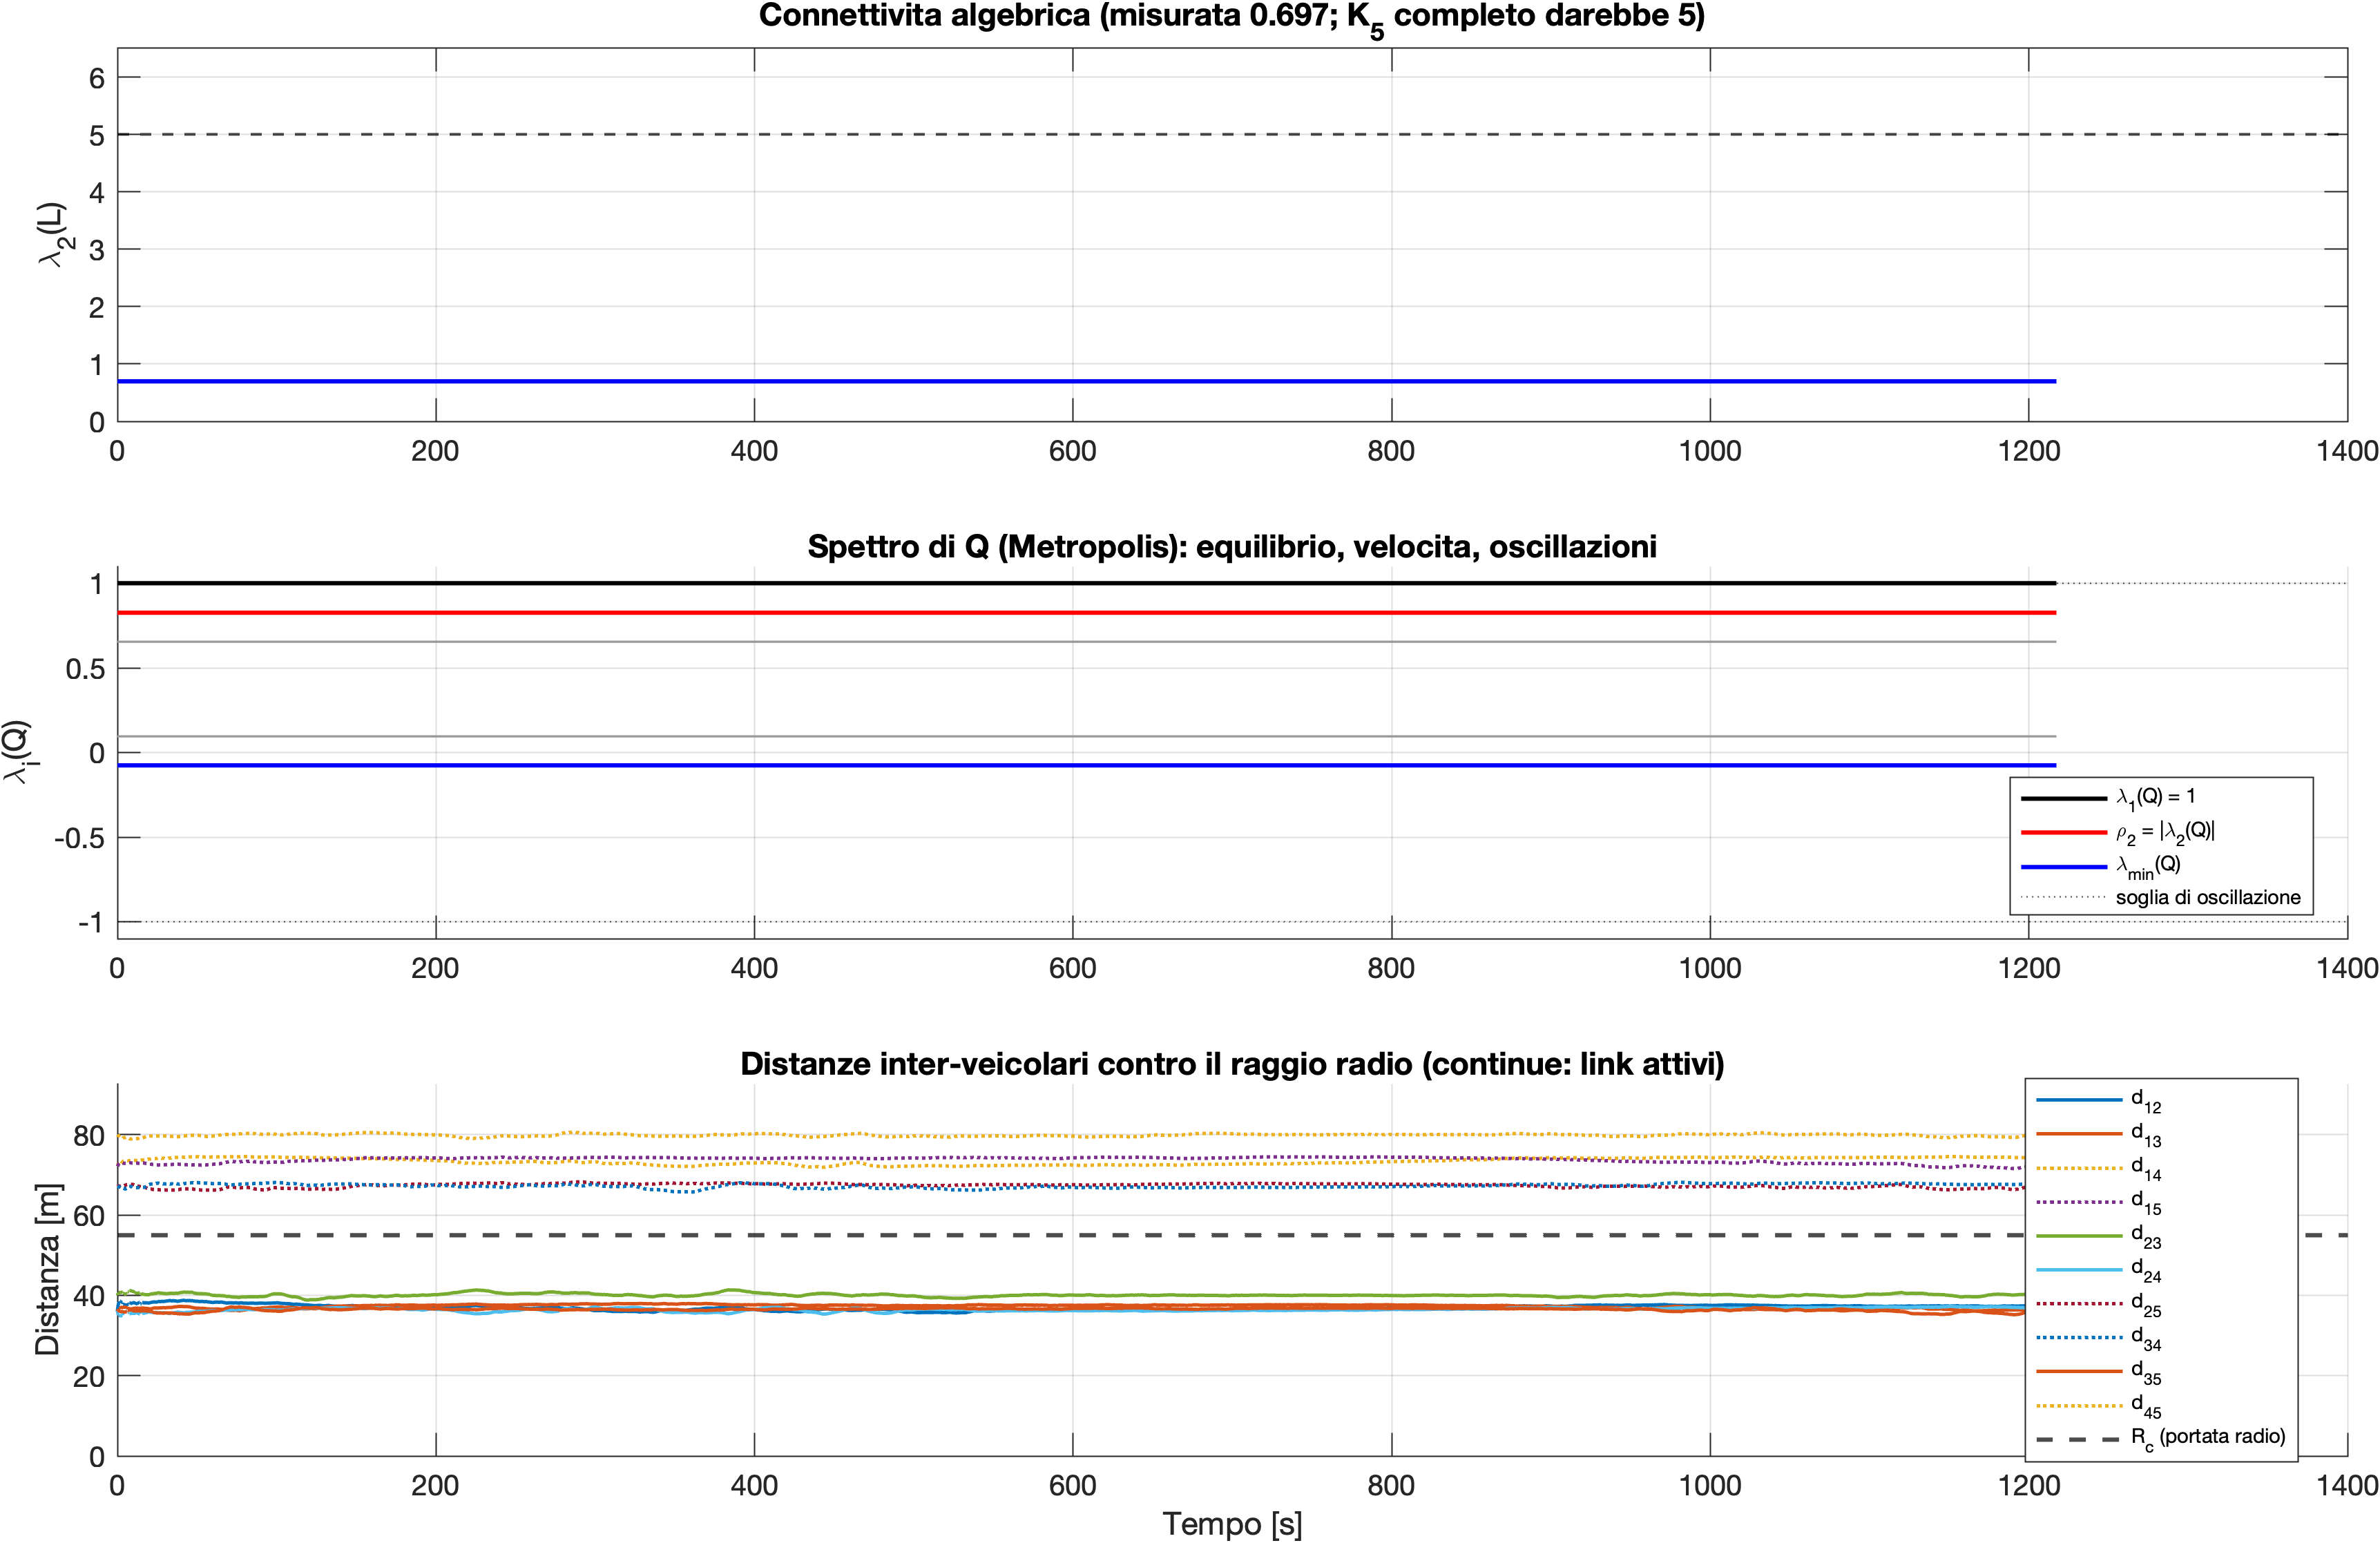
\includegraphics[width=0.74\textwidth]{figure/7_grafo_comunicazione.png}
\caption{Diagnostics of the communication graph. At the top the algebraic
connectivity $\lambda_2(L)$ and the number of active edges; in the middle the
spectrum $\lambda_i(Q)$ of the Metropolis matrix; at the bottom the ten
inter-vehicle distances compared with the radio radius (black dashed line). The
five solid curves stay well below the threshold, the five dotted ones well
above: it is the gap between the two groups that makes the topology stable
despite the formation error. The figure comes from a single run, but it is
representative of all of them: in the Monte Carlo campaign these quantities do
not vary at all ($\lambda_2(L) = 0.6972 \pm 0.0000$,
$\rho_2 = 0.8257 \pm 0.0000$, active edges $5.00 \pm 0.00$), because they
depend on the geometry of the formation and not on the noise.}
\label{fig:grafo}
\end{figure*}

\subsection{Localization accuracy}

Over the complete mission the satellite coverage is distributed as follows: in
\textbf{52.9\%} of the time all five vehicles receive the GNSS, in
\textbf{37.8\%} the coverage is \emph{mixed} (at least one vehicle covered and
at least one in the dark) and in \textbf{9.4\%} no vehicle has coverage. The
three percentages vary by barely a tenth of a point between the repetitions,
because they depend on the map and not on the noise. The central band is the
most relevant one, because it is there that a blind vehicle can anchor itself
to a neighbour that still sees the satellites, and it is worth more than a
third of the mission only thanks to the scale of the formation: 60\,m deep
against the 45--85\,m radius of the shadow zones. With a formation a few metres
wide the five vehicles would always share the same coverage and the
collaborative scenario would never occur.

Table~\ref{tab:accuratezza} reports the mean absolute position error, separated
between stretches with GNSS coverage and stretches in a blind zone.

\begin{table}[t]
\centering
\caption{Mean absolute error (MAE) of position and trace of the covariance,
separated by coverage condition. Mean and standard deviation over 50
repetitions; the trace of the covariance does not depend on the realization of
the noise and its dispersion across the runs is zero to the fourth digit.}
\label{tab:accuratezza}
\begin{tabular}{lccc}
\toprule
\textbf{Vehicle} & \textbf{MAE GNSS [m]} & \textbf{MAE blind [m]} &
$\mathbf{tr(\Sigma_{pos})}$ \textbf{blind}\\
\midrule
V1 (Master, RTK)  & $0.073 \pm 0.001$ & $0.078 \pm 0.004$ & 0.0129 m$^2$\\
V2 (Slave)        & $0.350 \pm 0.030$ & $0.086 \pm 0.005$ & 0.0124 m$^2$\\
V3 (Slave)        & $0.364 \pm 0.035$ & $0.078 \pm 0.005$ & 0.0131 m$^2$\\
V4 (Slave)        & $0.361 \pm 0.036$ & $0.088 \pm 0.004$ & 0.0163 m$^2$\\
V5 (Slave)        & $0.361 \pm 0.030$ & $0.079 \pm 0.003$ & 0.0143 m$^2$\\
\bottomrule
\end{tabular}
\end{table}

\textbf{The Slaves estimate 4.3 times better in a GPS-denied zone than under
open sky}. It is not a paradox but the direct consequence of the comparison
between two sources of information: a NEO-M8N receiver at $\sigma = 2.0$\,m
that produces one fix per second, against at least three UWB anchors at
$\sigma_{uwb} = 0.5$\,m interrogated at 10\,Hz and geometrically well
distributed.
Between one GNSS fix and the next the Slave spends 90\% of the steps in pure
prediction, supported by AHRS and encoders, and the uncertainty grows.

Fig.~\ref{fig:covarianza} shows the same phenomenon on the plane of the
declared covariance, and it is the plot that summarizes the whole behaviour of
the system. The upper panel counts the absolute references available to each
vehicle; the lower one plots $\mathrm{tr}(\Sigma_{pos})$ on a logarithmic
scale. On entering the blind zone the trace \emph{goes down} from about
0.33\,m$^2$ to 0.012\,m$^2$, an \textbf{improvement of 27 times}, and rises
again on exit. The Master, which has RTK at 5\,Hz, remains instead almost
indifferent: its curve is the horizontal line at the bottom.

\begin{figure*}[t]
\centering
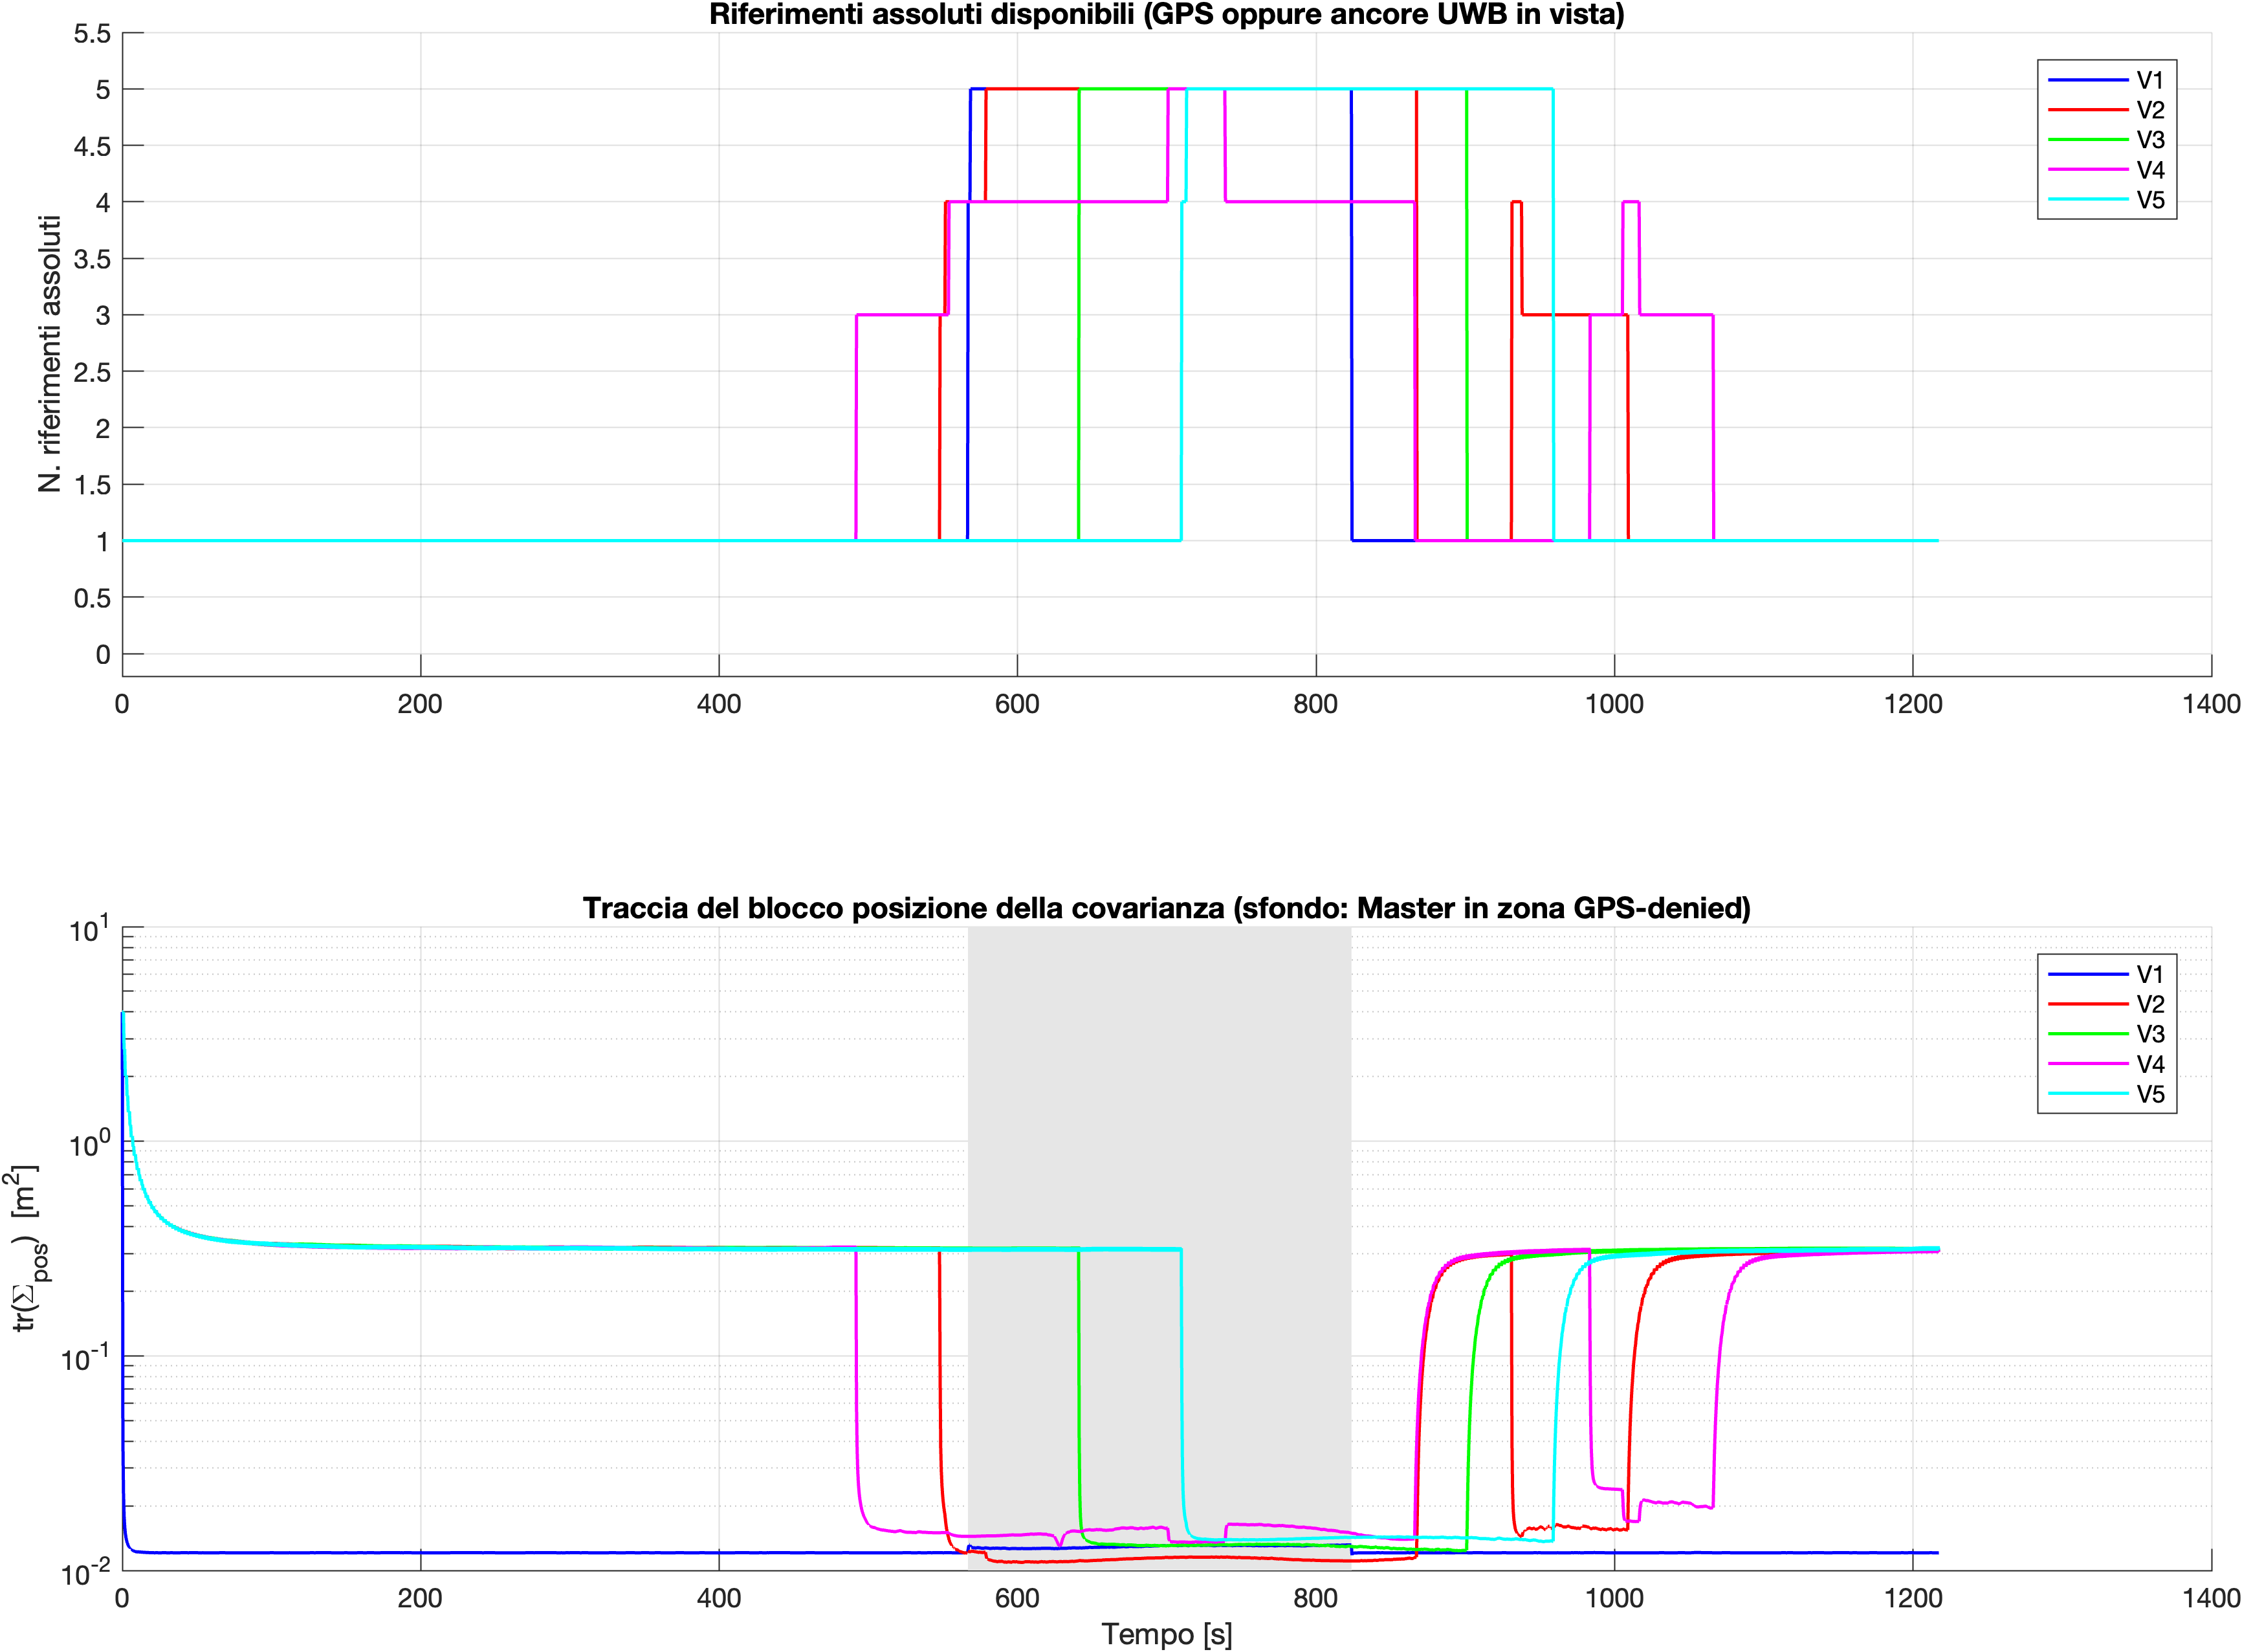
\includegraphics[width=0.74\textwidth]{figure/5_copertura_e_covarianza.png}
\caption{Sensor coverage and covariance. At the top the number of absolute
references (GNSS or UWB anchors in sight) for each vehicle; at the bottom the
trace of the position block of the covariance, on a logarithmic scale, with a
grey background in the stretches where the Master is in a GPS-denied zone. The
drop of more than an order of magnitude on entering the blind zone is the
central result of the work.}
\label{fig:covarianza}
\end{figure*}

The four Slaves turn out to be indistinguishable from one another, including
the two outer wings that have a single neighbour each: the sparse graph does
not degrade the localization, because in a blind zone the dominant reference
remains the fixed anchors and the collaborative ranging is an additional
contribution. The structure, in which local filters exchange estimates to
anchor each other, is the one analysed in~\cite{fontanelli2016}.

\subsection{Channel behaviour}

Table~\ref{tab:canale} summarizes the behaviour of the radio link.

\begin{table}[t]
\centering
\caption{Communication channel: required and measured values, mean and standard
deviation over 50 repetitions of about 244\,000 transmission attempts each.}
\label{tab:canale}
\begin{tabular}{lr}
\toprule
\textbf{Quantity} & \textbf{Measured value}\\
\midrule
Lost packets                           & $0.50 \pm 0.01$\% (required 0.5\%)\\
Quantized delay 0 / 1 / 2 steps        & 7\% / 87\% / 7\%\\
Mean age of the data used              & $\mathbf{100 \pm 0}$ \textbf{ms}\\
Maximum age per repetition             & $\mathbf{334 \pm 48}$ \textbf{ms}\\
Maximum age over the whole campaign    & 400 ms\\
Stability margin consumed              & 18\% (mean), 71\% (worst)\\
Theoretical limit~\eqref{eq:ritardo}   & 565 ms\\
Mobile anchor error                    & 0.002 m against $\sigma_{collab}=0.6$ m\\
\bottomrule
\end{tabular}
\end{table}

The maximum age of 400\,ms arises from two steps of delay plus two consecutive
losses, an event of probability $2.5\cdot10^{-5}$ per pair and per step. Over
244\,000 attempts the typical repetition reaches $334 \pm 48$\,ms, and the
400\,ms are the worst case observed over the whole campaign: it consumes 71\%
of the margin~\eqref{eq:ritardo}.

The measurable effect of the delay is on \textbf{speed, not on accuracy}: the
mission gets 13\% longer (from 1078 to $1218.0 \pm 0.2$\,s) because the
consensus acts on formation errors 100\,ms old, which is equivalent to reducing
the loop gain. The fleet stays stable but reacts more sluggishly. The 0.5\% of
loss is instead practically invisible: it raises the mean age by 0.005 steps,
that is half a millisecond.

A second effect, not related to the channel, concerns the steady-state speed.
Only the Master receives the velocity term $V_{rif}$ of the path following,
while the Slaves move only through the consensus. At steady state the formation
is rigid and moves entirely at velocity $v_f$; summing~\eqref{eq:consenso} over
all the $i$ and exploiting $\mathbf{1}^T L = 0$, the consensus term disappears:

\begin{equation}
N\,v_f = \sum_i V_{rif,i} \qquad\Longrightarrow\qquad
v_f = \frac{v_{cruise}}{N}
\label{eq:velflotta}
\end{equation}

The consensus is an \emph{internal} force and cannot move the centre of mass:
the only external push comes from the Master and is divided among all. The
verification is exact, $2.5/5 = 0.50$\,m/s against a measured value of
$0.443 \pm 0.000$\,m/s at steady state. Adding vehicles to a first-order
formation led by a Master slows it down in direct proportion; the solution is
to propagate $V_{rif}$ to the whole fleet, as reported among the future
developments.

\subsection{Distributed estimation of the terrain parameter}

The fleet runs a complete D-WLS round at every step, that is 12\,180 rounds
over the mission: a UWB exchange lasts about 1\,ms against the 100\,ms of the
step, and half of the step is reserved for this traffic, for a budget of
$q_{max} = 50$ cycles.

The distributed solution was compared at every round with the centralized WLS
computed on the simulator side. On the complete three-vehicle graph the
agreement is at machine precision ($1.5\cdot10^{-15}$); on the sparse graph the
discrepancy rises to $2.3\cdot10^{-8}$, because with $q$ truncated the
consensus is \emph{convergent but not exact}, and the residual disagreement
between the nodes is $7.2\cdot10^{-6}$. The only quantity that stays at machine
precision ($1.2\cdot10^{-15}$) is the invariance of the sum $\sum_i F_i$, and
this has a precise meaning: the columns of a doubly stochastic matrix sum to
one, therefore the consensus \emph{redistributes} the information without ever
duplicating it. It is the guarantee that the cycles of the graph do not trigger
\emph{double counting}.

\begin{table}[t]
\centering
\caption{Gain of the cooperation on the uncertainty of the parameter
$c_{terr}$, over 50 repetitions. In the network all the vehicles share the same
uncertainty, $8.04\cdot10^{-4}$. The last column is the dispersion of $v^2$
explored by each vehicle, which explains the third one.}
\label{tab:dwls_gain}
\begin{tabular}{lrcc}
\toprule
\textbf{Vehicle} & \textbf{alone} & \textbf{gain} & $\mathbf{std(v^2)}$\\
\midrule
V1 (Master)     & $9.04\cdot10^{-4}$ & $1.1 \pm 0.1\times$ & $0.108 \pm 0.039$\\
V2 (inner wing) & $3.44\cdot10^{-3}$ & $\mathbf{4.5 \pm 1.7\times}$ & $0.068 \pm 0.025$\\
V3 (inner wing) & $3.52\cdot10^{-3}$ & $\mathbf{4.7 \pm 1.9\times}$ & $0.067 \pm 0.029$\\
V4 (outer wing) & $6.19\cdot10^{-3}$ & $\mathbf{8.3 \pm 2.6\times}$ & $0.024 \pm 0.006$\\
V5 (outer wing) & $6.17\cdot10^{-3}$ & $\mathbf{8.2 \pm 2.3\times}$ & $0.024 \pm 0.005$\\
\bottomrule
\end{tabular}
\end{table}

Table~\ref{tab:dwls_gain} quantifies how much the cooperation is worth. The
correct comparison is not the condition number (the ratio between the largest
and the smallest eigenvalue), which gets slightly worse when adding Slaves even
in the presence of more information, but the covariance $(\sum_i F_i)^{-1}$,
which by the Loewner ordering can only decrease. The last column explains the
third one: the gain of each vehicle is the greater the less that vehicle, on
its own, explores different velocities. The Master, which has both the better
torque meter and the largest excursion, on its own would already get where the
network gets. \textbf{The network does not improve everyone in the same way: it
distributes to all the quality of the best instrumented member}, the same
structure as the RTK GNSS mounted on the Master alone.

The final estimate is $\mu_{terr} = 0.09010 \pm 0.00018$ and
$c_{terr} = 0.00457 \pm 0.00081$, against true values of 0.0900 and 0.00500,
with a relative error on the parameter vector,
$\lVert \hat x_{terr} - x_{terr}\rVert / \lVert x_{terr} \rVert$, equal to
$\mathbf{0.81 \pm 0.65\%}$. The two parameters are however not identified in
the same way: taken alone, $\mu_{terr}$ has an error of $0.17 \pm 0.15\%$,
while $c_{terr}$ reaches $\mathbf{14.2 \pm 11.6\%}$.

\textbf{The covariance declared by the D-WLS is however correct.} The
uncertainty that the algorithm declares on $c_{terr}$, $8.04\cdot10^{-4}$,
coincides with the dispersion actually observed across the 50 repetitions,
$8.14\cdot10^{-4}$: the ratio is \textbf{1.01}.

The estimates of the five vehicles stay indistinguishable from one another at
every round, as the consensus imposes.

The improvement with respect to the three-vehicle formation, with a relative
error going from 1.53\% to 0.81\%, does not come from going faster: the
five-vehicle fleet is in fact slower because of~\eqref{eq:velflotta}. It comes
from going at \emph{more different} velocities.
The outer wings are 40\,m from the axis against the 20\,m of the inner ones, so
in a curve their velocity departs from the Master's twice as much, and the
dispersion of $v^2$ that conditions the estimation problem grows. It is the
same lesson as the GDOP~\eqref{eq:gdop}: what counts is the geometric diversity
of the measurements, not their number.

\begin{figure*}[t]
\centering
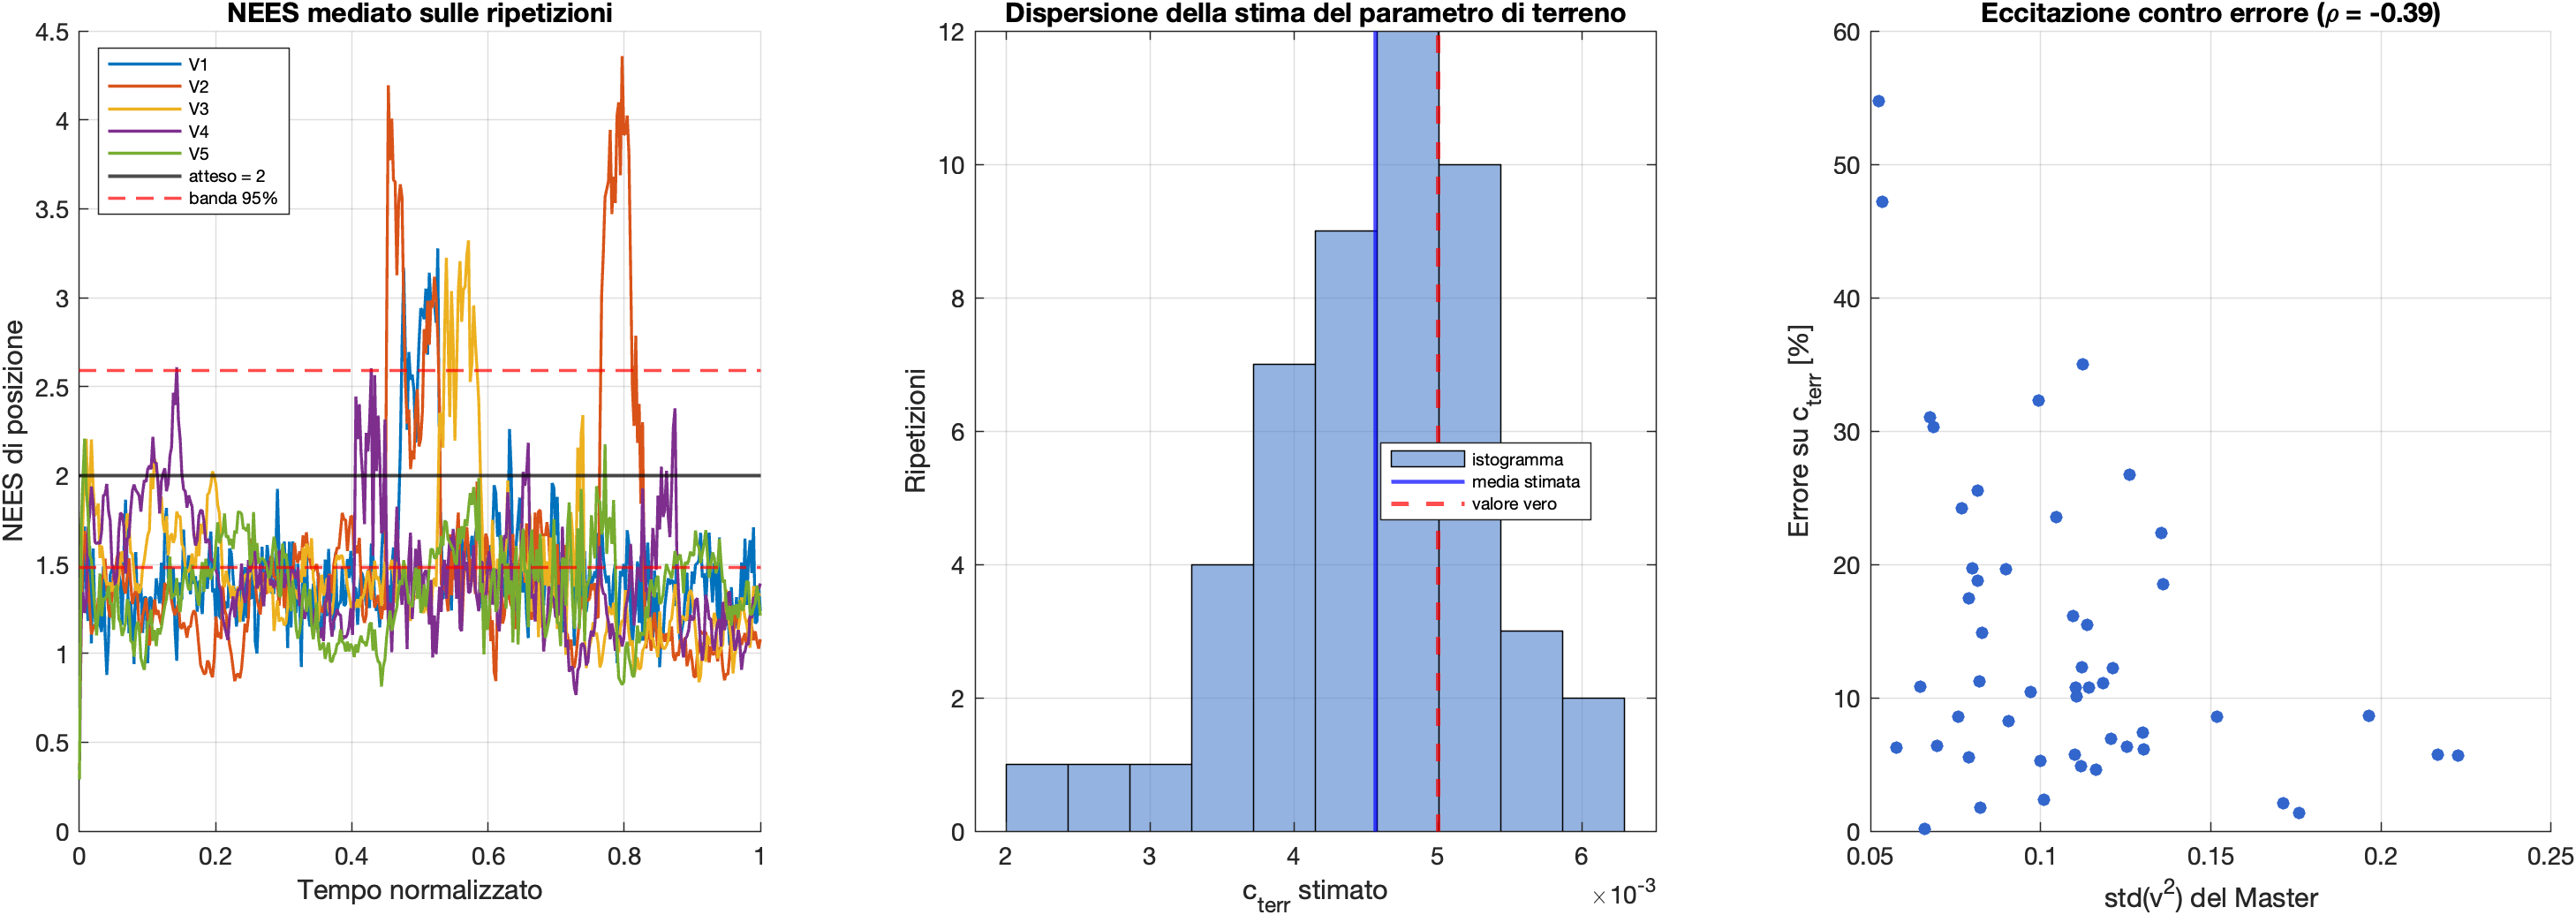
\includegraphics[width=0.92\textwidth]{figure/10_montecarlo_consistenza.png}
\caption{Outcomes of the Monte Carlo campaign over 50 repetitions. On the left
the position NEES averaged over the repetitions, with the expected value (2)
and the 95\% acceptance band; the grey background marks the window in which at
least one vehicle crosses a GPS-denied zone. In the middle the distribution of
the 50 estimates of the parameter $c_{terr}$, with the mean and the true value.
On the right every point is a repetition: on the abscissa the dispersion of
$v^2$ explored by the Master, on the ordinate the error committed on
$c_{terr}$.}
\label{fig:montecarlo}
\end{figure*}

The central panel of Fig.~\ref{fig:montecarlo} shows the distribution of the 50
estimates, shifted to the left of the true value, and the one on the right
explains its dispersion: the error on $c_{terr}$ is negatively correlated
($\rho = -0.39$) with the dispersion of $v^2$ explored by the Master. The
repetitions in which the lead vehicle crossed a wide velocity interval go below
10\% of error, those in which it stayed at almost constant velocity exceed
30\%. The conditioning of the network problem varies accordingly, from 34 to
373 across the repetitions. It is the same geometry of the information
discussed for the GDOP: two regression columns, $1$ and $v^2$, become collinear
when $v^2$ does not vary.

\subsection{Filter consistency}

With 50 repetitions consistency is verified in a statistical rather than
diagnostic sense. Denoting by $\tilde p$ the position error, the index
$\epsilon = \tilde p^T \Sigma_{pos}^{-1} \tilde p$ has an expected value equal
to its 2 degrees of freedom, and averaged over $M$ independent repetitions it
satisfies $M\bar\epsilon \sim \chi^2(2M)$. For $M = 50$ the two-sided 95\%
acceptance band is $[1.48,\ 2.59]$.

Over the whole mission the five vehicles give NEES between 1.36 and 1.55, and
four out of five fall below the lower end of the band. The filter is therefore
\textbf{consistent and significantly conservative}: it declares more
uncertainty than it has. It is the correct direction, because an estimate that
overstates its own uncertainty remains usable by whoever receives it while one
that understates it does not, and it is also the expected direction, given that
the process noise of Sec.~\ref{sub:cwna} is tuned on prudent values while the
simulated plant has ideal grip. Consistently, the samples outside the
$\pm 3\sigma$ envelope are 0.09\% against the 0.27\% expected.

\begin{table}[t]
\centering
\caption{Position NEES separated by coverage condition, over 50 repetitions.
The degree is the number of neighbours in radio range, and therefore the number
of collaborative measurements that the vehicle fuses in a blind zone.}
\label{tab:nees}
\begin{tabular}{lcccc}
\toprule
\textbf{Vehicle} & \textbf{degree} & \textbf{with GNSS} & \textbf{in blind zone} &
$\mathbf{\Delta}$\\
\midrule
V4 (outer wing) & 1 & $1.41 \pm 0.50$ & $1.53 \pm 0.16$ & $+0.12$\\
V5 (outer wing) & 1 & $1.34 \pm 0.40$ & $1.45 \pm 0.21$ & $+0.11$\\
V1 (Master)     & 2 & $1.37 \pm 0.09$ & $1.86 \pm 0.46$ & $+0.49$\\
V3 (inner wing) & 3 & $1.36 \pm 0.44$ & $1.85 \pm 0.60$ & $+0.49$\\
V2 (inner wing) & 3 & $1.24 \pm 0.32$ & $\mathbf{2.18 \pm 0.45}$ & $\mathbf{+0.94}$\\
\bottomrule
\end{tabular}
\end{table}

\textbf{Separating the two coverage conditions makes visible the limit declared
in Sec.~\ref{sec:conclusioni}.} Table~\ref{tab:nees} reports the NEES under open
sky and in a blind zone: the mean over the fleet goes from 1.35 to 1.77, and
the increase is ordered also in relation to the \textbf{degree of the node}. The two
outer wings, which have a single neighbour, move by barely $+0.11$ and $+0.12$;
the Master, with two neighbours, by $+0.49$; V2, which has three, by $+0.94$,
exceeding the expected value of 2.

The reading is direct. In a blind zone the filter fuses, besides the fixed
anchors, one distance measurement for every neighbour in range, and the pose of
that neighbour enters as if it were exactly known. Every collaborative
measurement therefore consumes a part of the conservativeness margin, in
proportion to their number. The filter stays inside the acceptance band, so it
does not become inconsistent, but the campaign shows that the margin thins out
exactly where and by the amount that the theory predicts. It is the
experimental justification of the Covariance Intersection proposed among the
future developments.

%=========================================================================
\section{Conclusions and future developments}
\label{sec:conclusioni}
%=========================================================================

The work has led to a working decentralized architecture for the localization
and formation control of a fleet of snow groomers in a hostile environment,
validated on a simulator that includes GPS-denied zones, UWB infrastructure, an
incomplete communication graph, sensors at their real frequencies and a channel
with delay and losses.

\subsection{Demonstrated benefits}

\begin{itemize}
\item \textbf{The UWB infrastructure more than compensates for the GNSS.} In a
      blind zone the trace of the covariance goes down by a factor of 27: five
      anchors at $\sigma_{uwb} = 0.5$\,m beat a receiver at $\sigma = 2.0$\,m and
      1\,Hz.
\item \textbf{Cooperation makes a locally singular problem solvable.} No
      vehicle identifies the two terrain parameters alone, having an
      instantaneous information matrix of rank 1 out of 2. The network
      distributes to all the quality of the best instrumented member, with
      gains up to 8$\times$ on the uncertainty.
\item \textbf{The spectral quantities are design tools.} The connectivity
      $\lambda_2(L)$ dimensions the consensus gain and the spectral radius
      $\rho_2$ the number of communication cycles.
\item \textbf{Combining delay and losses into the age of the data} made it
      possible to treat the non-ideal channel without timestamping or buffers.
\item \textbf{The repetition over 50 campaigns separates the properties of the
      system from the fluctuations of the noise.} Localization, channel and
      graph turn out stable to within a few percentage points, while the
      estimation of the terrain parameter reveals itself to be much more
      dispersed than a single run would suggest.
\end{itemize}

\subsection{Known limits and possible solutions}

\begin{itemize}
\item \textbf{The filter is optimistic on the collaborative measurement}, and
      the campaign measures it: the NEES grows in a blind zone in proportion to
      the number of neighbours fused (Table~\ref{tab:nees}). The $R$ of the
      ranging between vehicles contains only the sensor noise and ignores the
      uncertainty $\Sigma_j$ of the neighbour; worse, along the cycles of the
      graph what a node emits comes back to it after a few hops and re-enters
      its filter as new data (\emph{rumor propagation}), so the estimates
      become correlated in an unknown way and imposing zero correlation
      understates the covariance. \emph{Solution:} the Covariance
      Intersection described below.
\item \textbf{The switching architecture has a cost.} The UWB branch is
      activated only inside the blind zones: a Slave under open sky, in 90\% of
      the steps without a GNSS fix, does not use the anchors even though it has
      them in range, and pays 0.35\,m of error where it would pay 0.08.
      \emph{Solution:} condition the use of the anchors on their visibility
      rather than on the absence of GNSS; the EKF with variable $C_k$ already
      supports it.
\item \textbf{The formation slows down as $N$ grows}, because
      of~\eqref{eq:velflotta}, since only the Master receives the velocity
      reference. \emph{Solution:} propagate $V_{rif}$ forward to the whole
      fleet, or move to the second-order consensus described below.
\item \textbf{The regressor of the D-WLS is uncertain.} The row
      $C_i = [1\ \ \hat v_i^2]$ uses the estimated velocity, the only one
      available on board, and a noisy regressor attenuates the slope towards
      zero (\emph{errors-in-variables}). The campaign confirms it: the mean of
      the 50 estimates of $c_{terr}$ is $0.00457$ against a true value of
      $0.00500$, that is a systematic shortfall of 8.6\%, consistent in sign
      with the expected attenuation.
      \emph{Solution:} Reweighting of $R_i$ with the variance of $\hat v_i$?
\item \textbf{Grip is ideal}, the least defensible assumption for a tracked
      vehicle on snow. \emph{Solution:} the slip model described below.
\end{itemize}

\subsection{Future developments}

\textbf{Consistent fusion through Covariance Intersection.} It is the answer to
the first limit listed. The CI \cite{julier1997} fuses two estimates by
weighting the inverses of their covariances with $\gamma$ and $1-\gamma$, and
guarantees a covariance that upper bounds the real one \emph{for any} cross
correlation, without having to know it:
\begin{equation}
\Sigma^{-1} = \gamma\,\bar\Sigma^{-1} + (1-\gamma)\,C^T R^{-1} C
\label{eq:ci}
\end{equation}
where $\bar\Sigma$ is the a priori covariance of the vehicle and
$\gamma \in [0,1]$ is chosen by minimizing a measure of the size of $\Sigma$.
The classical CI however fuses two estimates of the \emph{same} quantity, while
here the neighbour transmits an estimate of its \emph{own} state.
The intervention also requires extending the exchanged packet from the position
alone to the pair $(\hat p_j, \Sigma_j)$, and the two modifications have to be
introduced \emph{together}: using $\Sigma_j$ to inflate $R$ while keeping the
standard Kalman gain would treat the uncertainty of the neighbour as
\emph{independent} noise, which is exactly the \emph{double counting} to be
avoided.

\textbf{Second-order consensus.} The law~\eqref{eq:consenso} is first order: it
acts on the position alone and assumes that the vehicle instantaneously reaches
the commanded velocity. By bringing the velocity too into the consensus state,
and exchanging both, three advantages would be obtained: the velocity reference
would propagate through the network instead of staying confined to the Master,
eliminating the slowdown $v_{cruise}/N$ of~\eqref{eq:velflotta}; the Master
would stop being a single point of failure, since every agent would have its
own desired position on the path; and the model would be faithful to the real
dynamics of the vehicle, which is a double integrator.

\textbf{Slip modelling.} The ground truth would go from $v^{true} = v^{cmd}$ to
a law $v^{true} = f_{slip}(v^{cmd}, x^{true}, \text{terrain})$, with three
consequences: the encoder model~\eqref{eq:enc} takes on a \emph{systematic}
error, because the encoders measure the velocity of the tracks and not that of
the vehicle; the process noise has to be retuned by activating the adaptive law
$q_a(v) = q_{a0} + k_{terreno}\,v^2$; and the parameter identified by the D-WLS
becomes its natural input, given that the same structure $\mu + c\,v^2$ governs
both phenomena.

There also remains to be addressed the regime of high losses, in which the
topology really fragments and the graph has to be re-read in terms of
\emph{joint connectivity}: the network can be disconnected at every single
instant and still sustain the consensus, provided that over time the links
cover the whole fleet. The Monte Carlo campaign would then have to be repeated
on that regime, where what varies would no longer be the noise alone but the
topology itself.

\balance

%=========================================================================
\begin{thebibliography}{9}

\bibitem{fontanelli_notes}
D.~Fontanelli, \emph{Intelligent Distributed Systems --- Course Notes},
Universit\`a degli Studi di Trento, 2024/2025.

\bibitem{thrun2005}
S.~Thrun, W.~Burgard, and D.~Fox, \emph{Probabilistic Robotics}.
Cambridge, MA: MIT Press, 2005.

\bibitem{barshalom2001}
Y.~Bar-Shalom, X.~R.~Li, and T.~Kirubarajan, \emph{Estimation with
Applications to Tracking and Navigation}. New York: Wiley, 2001.

\bibitem{olfati2004}
R.~Olfati-Saber and R.~M.~Murray, ``Consensus problems in networks of agents
with switching topology and time-delays,'' \emph{IEEE Trans. Automat. Contr.},
vol.~49, no.~9, pp.~1520--1533, Sep.~2004.

\bibitem{xiao2004}
L.~Xiao and S.~Boyd, ``Fast linear iterations for distributed averaging,''
\emph{Systems \& Control Letters}, vol.~53, no.~1, pp.~65--78, 2004.

\bibitem{khatib1986}
O.~Khatib, ``Real-time obstacle avoidance for manipulators and mobile
robots,'' \emph{Int. J. of Robotics Research}, vol.~5, no.~1, pp.~90--98, 1986.

\bibitem{julier1997}
S.~J.~Julier and J.~K.~Uhlmann, ``A non-divergent estimation algorithm in the
presence of unknown correlations,'' in \emph{Proc. American Control
Conference}, Albuquerque, NM, 1997, pp.~2369--2373.

\bibitem{fontanelli2016}
D.~Fontanelli, D.~Macii, P.~Nazemzadeh, and L.~Palopoli, ``Collaborative
Localization of Robotic Wheeled Walkers using Interlaced Extended Kalman
Filters,'' in \emph{Proc. IEEE Int. Instrumentation and Measurement Technology
Conference (I2MTC)}, Taipei, Taiwan, May 2016, pp.~1--6.

\end{thebibliography}

\end{document}
